\documentclass[final,3p,times,twocolumn,authoryear]{elsarticle}

\usepackage[T1]{fontenc}
\usepackage[utf8]{inputenc}
\usepackage[english]{babel}
\usepackage{amsmath,amssymb}
\usepackage{booktabs}
\usepackage{xcolor}
\usepackage{glossaries}
\usepackage{array}
\usepackage{multirow}
\usepackage{varwidth}
\usepackage{tabularx}
\usepackage{url}
\usepackage{subcaption}

\newcommand{\warn}[1]{{\color{red} {#1}}}
\newcommand{\verify}[1]{{\color{blue} {#1}}}
\newcommand{\remarks}[2]{{\color{red} #1\ (\textit{#2})}}

\journal{International Journal of Forecasting}

\begin{document}

\begin{frontmatter}

\title{ForeSight: Time Series Forecasting with Temporal Embeddings and Weightless Neural Networks}


\begin{abstract}
Time series forecasting is essential in scientific and applied areas, requiring methods that handle complex dynamics, nonlinear patterns, and heterogeneous data. Despite advances in machine learning, particularly deep learning, limitations remain in computational efficiency and generalization across diverse scenarios. This work proposes ForeSight, a hybrid method that integrates temporal embeddings with a weightless neural network (WNN), using latent representations to capture sequential dependencies. ForeSight is integrated into the open-source TSPredIT package, which supports preprocessing, optimization, reproducibility, and experimental comparison. We developed an evaluation protocol that compares ForeSight with traditional and selected state-of-the-art methods, including statistical methods, machine learning methods, and time series foundation models across heterogeneous domains and frequencies. Results indicate accuracy gains over the baseline WNN, with competitive performance against reference methods and lower computational cost than more complex alternatives. These findings highlight ForeSight's potential when computational efficiency and generalization are required, while its integration into TSPredIT supports reproducible and systematic comparisons.
\end{abstract}

\begin{keyword}
time series, forecasting, temporal embeddings, weightless neural networks, WiSARD, machine learning, open-source software
\end{keyword}

\end{frontmatter}
\thispagestyle{plain}


\section{Introduction}
\label{sec_introdction}


Time series arise naturally in contexts where phenomena are observed and recorded over time. Forecasting uses the information available up to a given instant to estimate subsequent behavior \citep{han_data_2012, hyndman_forecasting_2021, gujarati_essentials_2021}.

Historically, statistical methods dominated time series forecasting and proved effective in capturing linear and stationary structures \citep{box_time_2015, shumway_time_2017}. However, these approaches have limitations for series characterized by nonlinearity, high variability, and structural changes. With increased computational capacity and greater data availability, machine learning (ML) algorithms gained prominence, particularly artificial neural networks (ANNs), which are capable of capturing complex and nonlinear relationships \citep{haykin_neural_2009, hyndman_forecasting_2021}. This evolution expanded the boundaries of time series forecasting, albeit introducing challenges related to algorithmic efficiency and interpretability \citep{schmidhuber_deep_2015, makridakis_statistical_2018}.

In recent years, advances in natural language processing have led to the development of time series foundation models (TSFMs). These models are pretrained on large \textit{corpora} of heterogeneous series spanning different domains, frequencies, and scales. As a result, they can perform inference in unseen scenarios without requiring specific adjustments \citep{gruver_large_2023}. Temporal embeddings support their performance by transforming time series into expressive vector representations in latent space. These vectors capture short- and long-term dependencies and abstract complex dynamics, adapting to changes in data regimes \citep{trirat_universal_2026, irani_positional_2026}. Thus, the use of embeddings is a promising alternative for representing temporal dependencies, especially under nonstationarity \citep{lim_time_2021, trirat_universal_2026}.

Architectures such as weightless neural networks (WNNs) offer an approach distinct from ANNs because they are not based on neurons nested in layers, but on binary inputs (retinas) and addressed memories that store observed patterns. This structural simplicity leads to low computational cost and fast training while preserving generalization ability across several tasks \citep{aleksander_abrief_2009}. Although they have been successfully applied to classification and pattern recognition \citep{franca_advances_2014}, their use for forecasting future values remains underexplored. The studies examined in this work treat sequential data statically, using simple retina representations based on column charts \citep{desouza_fast_2011} or exact matches \citep{alhassan_using_2011}, limiting their ability to capture temporal dependencies. Finally, these studies are restricted to isolated applications and do not compare with state-of-the-art methods, preventing an assessment of their competitiveness.

This work presents \textit{ForeSight}, a method that integrates temporal embeddings with a WNN to address the lack of specialized mechanisms for handling time-series particularities through expressive latent representations that capture complex dynamics. Instead of operating directly on sliding windows, ForeSight projects temporal contexts into latent representations and uses them as the basis for the binary retinas processed by the WNN. The method is integrated into the open-source TSPredIT (Time Series Prediction with Integrated Tuning) package \citep{anonymous_2023}, which offers a unified environment for data preparation, hyperparameter tuning, forecasting strategy definition, evaluation, and experiment logging, favoring reproducibility and systematic comparison of different methods.

The main contributions of this work are (i) the definition of ForeSight as a forecasting method that combines temporal embeddings and WNNs, (ii) a broad empirical evaluation of temporal representation strategies and latent dimensions, comparing predictive performance and computational cost with classical, ML, deep learning, and TSFM-based reference methods across heterogeneous time series, (iii) a feature-based characterization of the temporal properties associated with ForeSight's performance gains, and (iv) the open-source integration of ForeSight into TSPredIT, providing a reproducible workflow for execution, comparison, and experiment logging.

We seek to answer the following questions (RQs): \textit{RQ1}: How does ForeSight compare with established forecasting methods in terms of predictive performance and computational efficiency across heterogeneous time series? \textit{RQ2}: How do the temporal encoding technique and latent dimension affect the trade-off between ForeSight's predictive performance and computational cost? \textit{RQ3}: Which time series characteristics are associated with ForeSight's largest performance gains? To this end, we designed a comprehensive evaluation protocol that includes preprocessing, hyperparameter optimization, forecasting scenario definition, and computation of error, runtime, and estimated energy consumption.

We conducted experiments on hundreds of heterogeneous series involving challenges such as short series, nonstationarity, and varied granularity to measure predictive performance and computational efficiency under different conditions. The results show that ForeSight improves predictive performance over the baseline method while maintaining comparable computational cost in compact configurations. Compared with select state-of-the-art methods, ForeSight is competitive in evaluated scenarios, showing a favorable balance between predictive accuracy, runtime, and estimated energy consumption.

The remainder of this paper is organized into six sections. Section~\ref{sec_background} presents the theoretical background needed to understand the method, discussing time series principles and the general forecasting process, followed by the main statistical, ML, and TSFM methods and the foundations of temporal embeddings. Section~\ref{sec_related} reviews related work, presenting studies that investigated the use of WNNs in regression and highlighting the main gaps identified. Section~\ref{sec_foresight} presents ForeSight, which uses latent representations and a WNN for time series forecasting, discusses its design details, and explains how the method mitigates known limitations. Section~\ref{sec_framework} describes the integration of ForeSight into TSPredIT and details the evaluation workflow used to structure the comparative assessment of forecasting methods. Section~\ref{sec_experiments} presents the experimental evaluation, describing the setup, data selection and partitioning, applied techniques, and results. Finally, Section~\ref{sec_conclusion} summarizes the work's main contributions, highlights the limitations found, and proposes directions for future research.

\section{Background}
\label{sec_background}

\subsection{Time Series}
\label{sec_timeseries}

Time series are a particular type of data that record the evolution of one or more variables over time. The natural (chronological) ordering of observations is a fundamental part of the series because it allows the dynamics of the phenomena that generated it to be captured and modeled \citep{box_time_2015, kontopoulou_areview_2023}. Mathematically, a time series $X$ can be represented by a vector of real numbers $\{x_1, \dots, x_T\}$, where $T = |X|$ denotes its size in terms of the total number of observations, and $x_t$ is the observation recorded at time instant $t \in \{1, \dots, T\}$ \citep{shumway_time_2017}. This notation expresses the sequential nature of the data, such that $x_1$ is the oldest observation in the series and $x_T$ is the most recent.

The series addressed in this work are univariate, discrete, and recorded at constant intervals. In this case, adjacent observations are often correlated or dependent, meaning that the value at a given moment may be influenced by past values \citep{han_data_2012}. In addition, an observation can be represented as the sum of three components \citep{hyndman_forecasting_2021}: $x_t = \tau_t + \lambda_t + \varepsilon_t$, where $\tau_t$ represents the trend component, $\lambda_t$ the seasonal component, and $\varepsilon_t$ the residual term (or random component).

Time series can also be described by properties (features) extracted directly from their observations. These descriptors summarize aspects of the distribution of series values, linear and nonlinear temporal dependencies, the behavior of consecutive-observation variations, and spectral characteristics such as periodicity and frequency content. Such a feature- and moment-based representation \citep{lubba_catch22_2019} compactly summarizes the generating stochastic process and is widely used to characterize, classify, and cluster temporal data, especially across domains and varying series lengths \citep{fulcher_highly_2014}.

Another distinction in time series analysis is related to the stationarity of the process, which occurs when the mean ($\mathbb{E}[X] = \mu$) and variance ($\texttt{Var}(X) = \mathbb{E}[(X-\mu)^2] = \sigma^2$) are constant and do not depend on time \citep{shumway_time_2017, gujarati_essentials_2021}. In addition, the autocovariance of the lagged series $X_{t-l}$ and $X_t$, expressed by $\gamma(X_t, X_{t-l})$, depends only on the lag $l$ between them \citep{ogasawara_event_2025}. One approach to handle nonstationarity is differencing, which computes differences between consecutive values of the series. Applying it produces a transformed series that tends to have properties closer to stationarity \citep{salles_nonstationary_2019}.

\subsection{Time Series Forecasting}
\label{sec_process}

Time series forecasting seeks to model the dependence between past and future values of the series, assuming that historical observations contain useful information for estimating subsequent values \citep{han_data_2012}. The information available up to a given instant is used to infer the behavior of the series in the following periods. The reliability of the estimates depends on factors such as the consistency and coverage of the data used, the model's ability to capture relevant patterns in the series, and the validity of the assumptions adopted about the nature of the generating stochastic process \citep{hyndman_forecasting_2021, gujarati_essentials_2021}.

Error metrics are used to quantify forecasting accuracy relative to actual observations and can be computed in absolute, percentage (relative), or normalized form. Let $\mathcal{T} = \{t+1, \dots, T\}$ be the set of instants in the test period, and let $x_t$ and $\hat{x}_t$ be the actual and predicted values, respectively, associated with period $t \in \mathcal{T}$. The mean absolute error computes the average absolute error, offering a robust view of the overall error. The mean squared error (MSE) calculates the average squared error, penalizing larger deviations and being more sensitive to outliers. The root mean squared error, defined as the square root of the mean squared error, expresses the error in the same unit as the predicted variable \citep{hyndman_forecasting_2021}. Other metrics widely used include the coefficient of determination, which measures the proportion of variance in the observed data explained by the model, and the symmetric mean absolute percentage error (sMAPE), which quantifies deviations as a percentage. This enables cross-domain interpretation and comparison and is used in time series forecasting competitions \citep{koning_them3_2005, makridakis_m5_2022}.

Once the adopted metric(s) have been defined, statistical significance tests, such as Student's $t$-test for paired samples (parametric, for normal distributions), the Wilcoxon test (nonparametric), or analysis of variance, can be applied to verify whether differences in model results are statistically significant \citep{montgomery_applied_2011}, typically rejecting the null hypothesis when the $p$-value is $\leq 0.05$. For the Wilcoxon test, the effect size is calculated as $r=|Z|/\sqrt{N}$ and is therefore nonnegative \citep{tomczak_need_2014}. Values below 0.3, from 0.3 to below 0.5, and 0.5 or above indicate low, moderate, and high effect magnitudes, respectively.

For comparison across multiple time series, ranking-based evaluation procedures are also commonly adopted \citep{koning_them3_2005, makridakis_m5_2022}. In these cases, models are ordered individually within each dataset according to the adopted evaluation metric, assigning first place to the best-performing model, second place to the next model, and so on. The average position obtained by each model across all tested sets is then computed. Thus, methods that present consistently better results tend to obtain lower average rankings, providing a global comparison that is less sensitive to the scale of the metric used and to the particularities of each dataset.

\subsection{Main Forecasting Methods}
\label{sec_models}

According to the assumptions made about the data-generating process, predictive methods can be divided into rigid and flexible methods \citep{salles_framework_2017}. The former assume a predefined structure to represent the relationship between variables, as in statistical methods. Although they have low computational cost and high interpretability, making them attractive in contexts with computational constraints, these approaches tend to perform poorly when modeling more complex or nonlinear patterns \citep{kontopoulou_areview_2023}.

Linear regression assumes that the response variable can be represented as a linear combination of the input variables. Polynomial regression extends this formulation by including powers of the input variables, increasing the model's flexibility to represent nonlinear relationships \citep{salles_framework_2017}. The transition to the autoregressive (AR) model occurs when, instead of external variables, the series' own past values are used as predictors \citep{shumway_time_2017}.

Complementing this approach, moving average (MA) models assume that the current value of the series depends on linear combinations of past random errors \citep{shumway_time_2017}. Combining AR and MA processes yields the autoregressive moving average (ARMA) model, which integrates the former's ability to represent temporal dependencies with the latter's ability to capture the effects of past shocks. The autoregressive integrated moving average (ARIMA) model extends ARMA by applying differencing to achieve stationarity before fitting the model. In an ARIMA($\rho, d, q$) model, parameter $\rho$ represents the order of the autoregressive component, $d$ indicates the number of differencing operations applied, and $q$ corresponds to the order of the moving average component \citep{box_time_2015}.

Unlike statistical approaches, ML algorithms for time series forecasting are flexible methods because they require fewer assumptions about the behavior of the series \citep{salles_framework_2017}. This flexibility stems from their data-driven nature, allowing them to capture nonlinear relationships and complex interactions, as well as to adapt better to dynamic patterns and structural changes in the data \citep{han_data_2012, kontopoulou_areview_2023}. Although they may require a larger volume of observations and greater computational capacity, the models show competitive or superior performance when applied to time series with high variability or nonstationary behavior \citep{makridakis_statistical_2018, hyndman_forecasting_2021}.

Predictions are obtained by using as input a sliding window (SW) of size $s$ containing the most recent observations to predict the subsequent value at $t+1$ \citep{han_data_2012}. Let $\texttt{seq}_{i,s}(X)$ be the subsequence of size $s \geq 1$ obtained from $X$ that ends at position $i$, that is, $\{x_{i-(s-1)}, x_{i-(s-2)}, \dots, x_i\}$, where $s \leq i \leq |X|$. This process consists of segmenting the original series into multiple SWs that move through time with partial or total overlap. Mathematically, an SW of $X$ with size $s$ is a function $\text{\texttt{sw}}_s(X)$ that produces a matrix $W$ of size $m \times s$, in which each row $w_i \in W$ is the $i$-th subsequence of size $s$ obtained from $X$ and $m = |X| - s + 1$ \citep{ogasawara_event_2025}.

The $k$-nearest neighbors ($k$NN) method is nonparametric and makes predictions based on the similarity between the input window and historical samples, selecting the $k$ nearest neighbors according to a distance metric and aggregating their following values to obtain the prediction \citep{yakowitz_nearest_1987}. Support vector regression (SVR) is a method derived from support vector machines for regression tasks, fitting a function within a tolerance margin around the observed values and penalizing only deviations that exceed this limit \citep{vapnik_support_1996}. Through kernel functions, such as linear, radial, or sigmoid kernels, SVR can model nonlinear relationships between variables \citep{haykin_neural_2009}. In time series, the input variables correspond to lags of the series itself, whose number, together with the kernel, violation cost, and tolerance margin, influences the balance between flexibility and the model's generalization capacity \citep{cao_support_2003}.

The random forest regressor (RFR) is an ensemble model of decision trees in which multiple predictors are aggregated to increase the stability and accuracy of predictions \citep{breiman_random_2001}. After windowing the series, each tree is trained on a random sample of SWs with replacement, and at each split only a random subset of lags is considered, promoting diversity among the trees and reducing variance and susceptibility to overfitting. The prediction is obtained by averaging the tree outputs, and its performance is mainly influenced by the number of trees and the minimum size of terminal nodes, which control the stability and complexity of the model \citep{breiman_random_2001}.

The multilayer perceptron (MLP) is a fully connected ANN in which each neuron in one layer is connected to the neurons in the following layer \citep{bishop_neural_1995}. Its ability to model nonlinear relationships depends on the number of neurons, while the decay rate and learning rate control regularization and the speed of weight updates, respectively \citep{haykin_neural_2009}. MLP networks perform well in time series forecasting, including in complex and nonstationary scenarios \citep{aslanargun_comparison_2007, weytjens_cash_2019}, but they assume underlying dynamics that are invariant over time and may incur high computational cost due to iterative gradient-based training \citep{huang_extreme_2006, makridakis_statistical_2018}.

The extreme learning machine (ELM) is an ANN distinguished by computational efficiency and fast training \citep{huang_extreme_2006}. Unlike feedforward networks, it has a single hidden layer whose input weights are assigned randomly and remain fixed throughout the learning process. The activation function applied in this layer transforms the input signals, introducing nonlinearity that enables the network to model complex relationships in the data. Thus, iterative adjustments until convergence are not required. The output weights, in turn, are computed analytically, which makes training faster \citep{huang_extreme_2006}.

Deep learning (DL) algorithms represent an evolution of ANNs by employing multiple layers capable of learning representations at different levels of abstraction, increasing the ability to model complex and nonlinear patterns \citep{schmidhuber_deep_2015}. One-dimensional convolutional networks (Conv1D) use filters that slide along the sequence to identify local patterns, acting as feature extractors relevant to forecasting \citep{larabenitez_temporal_2020}. Recurrent networks process sequential data by using past information to influence subsequent predictions \citep{schmidhuber_deep_2015}. Long short-term memory (LSTM) networks incorporate memory cells that preserve relevant information over longer periods, enabling the capture of short- and long-term dependencies \citep{hochreiter_long_1997}.

While conventional methods are fitted individually to a single dataset, TSFMs are pretrained on large \textit{corpora} of heterogeneous series from multiple domains, frequencies, and lengths, allowing them to learn general representations of temporal dynamics. This characteristic gives them high generalization capacity and the ability to perform inference without application-specific adjustments \citep{gruver_large_2023}. For this reason, they can also be considered flexible methods because they do not impose strict assumptions about the behavior of the series.

\subsection{Temporal Embeddings}
\label{sec_embeds}

A central aspect of TSFMs is the explicit representation of series structures through temporal embeddings \citep{trirat_universal_2026}. When the problem involves a single series $X$, this representation can be built from individual observations, subsequences, or SWs of $X$, which are treated as independent instances during model training. Initially, the function $\texttt{sw}_s(\cdot)$ is applied to series $X$, yielding the matrix $W_{m \times s} = \texttt{sw}_s(X)$, composed of $m$ consecutive windows of size $s$. Next, a transformation $f$ is applied to map each window $w_i \in \mathbb{R}^{1\times s}$ of $W$ into a vector representation of dimension $r$, that is, $f : w_i \mapsto \omega_i$, where $\omega_i \in \mathbb{R}^{1\times r}$ represents the embedding associated with window $w_i$. In matrix notation, this transformation produces $\Omega \in \mathbb{R}^{m \times r}$, whose rows correspond to the representations of the $m$ windows in $W$. For clarity, the following formulations consider that $t = 0, \dots, s - 1$ denotes the relative temporal position within the $i$-th window.

Embedding techniques can be grouped into two categories. The first comprises approaches based on fixed encodings, in which vector $\omega_i$ is obtained by a predefined function without parameter adjustment during training. In these cases, the transformation can be expressed as $\Omega = WP$, where $P \in \mathbb{R}^{s\times r}$ is the projection matrix used by the encoding technique \citep{irani_positional_2026}. The second category includes learnable encodings, in which a neural network learns a vector representation for each window contained in $W$. Thus, the encoding is represented by $\Omega = f_{\theta}(W)$, where $f_{\theta}$ denotes a function parameterized by the network weights $\theta$ \citep{trirat_universal_2026}.

Among fixed variants, positional encoding (PE) was developed to explicitly incorporate the position of sequence elements \citep{vaswani_attention_2017}. The elements of matrix $P$ are obtained according to Equation~\ref{eq_pe}, where $u = 0, \ldots,\lfloor r/2 \rfloor - 1$ indexes the pairs of embedding dimensions. Although efficient, PE uses a fixed sinusoidal basis and disregards the spectral characteristics of the time series \citep{irani_positional_2026}.

\begin{equation}
\label{eq_pe}
P_{t,2u} = \sin\left(\frac{t}{10000^{2u/r}}\right), \: P_{t,2u+1} = \cos\left(\frac{t}{10000^{2u/r}}\right)
\end{equation}

In Fourier encoding (FE), matrix $P$ is built from sine and cosine functions associated with a predefined set of frequencies $\{\nu_u\}$ distributed on a logarithmic scale. Each element determines a distinct harmonic component. Thus, patterns that appear at different temporal scales can be simultaneously incorporated into the embedding representation \citep{bloomfield_fourier_2018}. Equation~\ref{eq_fe} expresses this construction:

\begin{equation}
\label{eq_fe}
P_{t,2u} = \sin(2\pi \nu_u t), \: P_{t,2u+1} = \cos(2\pi \nu_u t)
\end{equation}

where $\nu_u$ corresponds to the frequency associated with the $u$-th harmonic component. However, adopting a deterministic set of frequencies restricts the diversity of the resulting sinusoidal projections, making representation quality directly dependent on this parameterization \citep{tancik_fourier_2020}.

In contrast, random Fourier features (RFF) introduce stochasticity into the temporal representation. Originally developed to approximate translation-invariant kernel functions through random projections onto Fourier bases \citep{rahimi_random_2007}, RFF can be adapted to construct a stochastic temporal basis by replacing the deterministic frequencies used in FE with random samples from a normal distribution, $\tilde{\nu}_u\sim\mathcal{N}(0,\sigma^2)$, where $\sigma$ controls their spread. The elements of $P$ are computed according to Equation~\ref{eq_rff} \citep{tancik_fourier_2020}:

\begin{equation}
\label{eq_rff}
P_{t,u} = \sqrt{\frac{2}{r}} \cos(\tilde{\nu}_u t+\xi_u)
\end{equation}

where $u = 0, \dots, r - 1$ indexes the embedding dimensions and $\xi_u\sim\mathcal{U}(0, 2\pi)$ represents a random phase drawn from the uniform distribution over the interval $[0, 2\pi]$. Each component $P_{t,u}$ corresponds to a different sinusoidal projection, making it possible to build temporal representations that are more adaptable to data characteristics \citep{rahimi_random_2007, tancik_fourier_2020}.

The Multiscale Random Fourier Features (MSRFF) technique extends this approach by employing $L$ distinct scales \citep{wang_onthe_2021, novelli_fast_2025}. Random frequencies are sampled from a normal distribution $\mathcal{N}(0,\sigma_\ell^2)$, with $\ell = 1, \dots, L$, producing sinusoidal projections at different levels of granularity. As a consequence, the generated embeddings become capable of simultaneously capturing short-, medium-, and long-term temporal patterns, increasing their ability to describe dynamics present in the original series. Matrix $P$ is obtained by combining the matrices $P^{(1)}, P^{(2)}, \dots, P^{(L)}$, whose elements are defined by Equation~\ref{eq_msrff} \citep{wang_onthe_2021}:

\begin{equation}
\label{eq_msrff}
P^{(\ell)}_{t,u} = \sqrt{\frac{2}{r}} \cos\!\left(\tilde{\nu}^{(\ell)}_u t + \xi^{(\ell)}_u\right)
\end{equation}

where $\tilde{\nu}^{(\ell)}_u\sim\mathcal{N}(0,\sigma_\ell^2)$ is the random frequency of the $u$-th component at the $\ell$-th scale, and $\xi^{(\ell)}_u\sim\mathcal{U}(0,2\pi)$ is the corresponding random phase. Since only the construction of $P$ is modified, the technique preserves low computational cost while incorporating information related to the periodicity of observations \citep{novelli_fast_2025}.

All techniques presented so far share a characteristic: matrix $P$ remains fixed regardless of the observed data. To overcome this limitation, learnable encodings learn the parameters of the transformation function $f$ applied to the windows of $W$ \citep{trirat_universal_2026}. One such approach is convolutional stochastic positional encoding (ConvSPE) \citep{liutkus_relative_2021}, which uses Conv1D to explore local dependencies among neighboring sequence elements \citep{larabenitez_temporal_2020} without relying on predefined sinusoidal components.

TS2Vec is one of the main learnable encoding techniques. The generated embeddings not only represent local patterns but also encode long-term dependencies by using a hierarchical contrastive strategy. Its architecture consists of a neural network that extracts the contextual representation at each instant $t$, providing flexibility to handle different temporal granularities efficiently \citep{yue_ts2vec_2022}.

The TS2Vec training process is based on hierarchical contrastive learning. Two overlapping contextual views are generated from each series through random cropping and timestamp masking. At each temporal resolution, the objective combines a temporal contrastive loss, which treats representations of the same timestamp in the two views as positive pairs and other timestamps as negatives, with an instance-wise contrastive loss, which contrasts representations from different series in the same batch. Successive max-pooling operations along the time axis repeat this dual objective at multiple resolutions, allowing the resulting representations to encode both local and long-range temporal information \citep{yue_ts2vec_2022}.

Another relevant technique in the context of learnable encodings is TRep, which seeks to enrich embeddings $\omega_{i,t}$ with explicit temporal information, giving latent space a more adaptive temporal structure \citep{fraikin_trep_2024}. More specifically, TRep introduces time-embeddings, which encode temporal properties such as trends, periodicities, and irregular variations from time instants. Different architectures can be used at this stage, such as dedicated ANNs. These time-embeddings are then combined with the embeddings of the series values through a convolutional network to form the final representation $\omega_{i,t}$. Thus, the embeddings produced by TRep reflect not only the context but also its local temporal structure around each instant $t$ \citep{fraikin_trep_2024}.

\subsection{\textit{Regression} WiSARD}
\label{sec_rew}

WNNs originated from the $n$-tuple architecture for binary pattern recognition, in which each neuron maps a subset of the input bits to form a tuple associated with a lookup table storing information about the classes observed during training. WiSARD (Wilkie, Stonham and Aleksander's Recognition Device) is one of the most prominent WNN architectures and was originally developed for black-and-white image recognition \citep{aleksander_wisard_1984}. Its basic unit is the discriminator, which consists of $N$ random-access memory (RAM) modules operating in parallel and a summation node $\Sigma$.

The input pattern, referred to as the retina, is represented as a binary vector of length $M$, with each position corresponding to a feature in the input image. Each RAM receives a tuple of $n = M/N$ pixels, where $n$ denotes the RAM size and determines the $2^n$ addressable memory locations, one for each possible combination of its $n$ binary inputs. During training, the memory locations addressed by the presented patterns are activated (set to 1). During inference, the summation node $\Sigma$ counts the number of RAMs whose addressed memory locations are active, thereby producing the discriminator's response \citep{aleksander_abrief_2009}. Building on WiSARD's memory structure, \citet{cardoso_clustering_2016} introduced a knowledge forgetting mechanism that removes addresses associated with outdated observations from discriminator nodes.

Despite their simplicity, WNNs involve a trade-off between tuple size and resource requirements, since the number of addressable locations in each RAM grows exponentially with tuple size. To address this issue, \citet{susskind_weightless_2022} proposed BTHOWeN, which uses counting Bloom filters and hardware-friendly hash functions to reduce model size and energy consumption while improving accuracy. From a different perspective, \citet{bacellar_differentiable_2024} introduced an architecture based on interconnected lookup tables, trained through an Extended Finite Difference technique for the approximate differentiation of binary values. The model also incorporates learnable mapping and reduction operations, as well as spectral regularization, expanding training possibilities and improving the accuracy and efficiency of WNN architectures.

The first efforts exploring the use of WNNs for regression tasks were introduced by \citet{kolcz_ntuple_1996}, who modified the $n$-tuple network to operate as a nonparametric estimator capable of approximating probability distributions and other deterministic functions. Each RAM position stores not only a counter for the number of accesses $c$, but also the sum of the $y$ values of a real-valued variable of interest, enabling estimates based on the mean \(\displaystyle \Big(\frac{\Sigma y}{\Sigma c}\Big)\). This approach is known as the $n$-tuple regressor.

Based on this concept, \citet{lusquino_prediction_2019, lusquino_extending_2020} present Regression WiSARD (ReW) as an extension of the WiSARD classifier for regression, associating real-valued outputs with binary input patterns. The network has a single discriminator whose RAMs consist of two-dimensional positions, as in the $n$-tuple regressor, initially set to 0. Thus, each RAM position accessed by a given input tuple is used to learn and represent numerical relationships from the samples observed during training.

The discriminator is trained with pairs $(\chi, y)$, where $\chi$ is an $M$-dimensional retina and $y$ is a real value associated with it, so that RAM positions are updated for each presented pattern. In Figure~\ref{fig_rew1}, the model receives an input pattern with $y = 4.7$. Training consists of incrementing the counter of the positions accessed by each tuple in the first RAM dimension ($\Sigma c$), while the other dimension (in blue) adds the value of $y$ to the sum stored so far ($\Sigma y$).

\begin{figure*}[!ht]
    \centering
    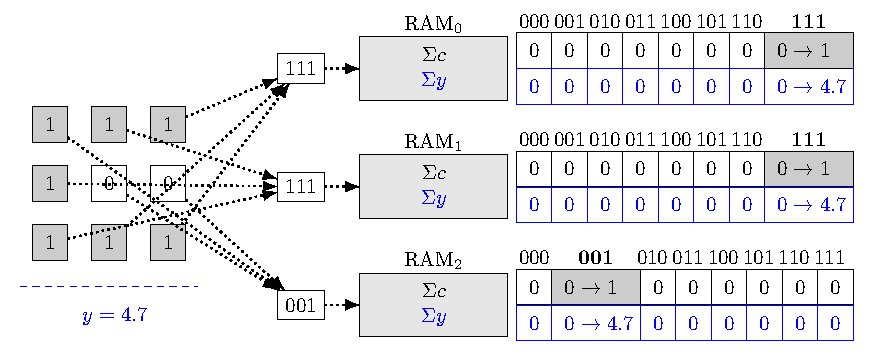
\includegraphics[width=0.75\textwidth]{fig_regwis1.pdf}
    \caption{Training ReW with the first sample}
    \label{fig_rew1}
\end{figure*}

In Figure~\ref{fig_rew2}, the procedure is repeated with another retina associated with $y = 3.1$. For $\text{RAM}_0$, a new address is accessed and its content is updated, while the remaining positions are unchanged. The other RAMs receive the same input tuple, causing their counters to be incremented again and their accumulated $y$ values to be increased with the new observation. Thus, identical patterns identified in the retina map their corresponding $y$ values to the same memory position \citep{lusquino_extending_2020}. This property is fundamental in the inference phase, allowing the estimate for a given retina to consider only the values accumulated by similar retinas.

\begin{figure*}[!ht]
    \centering
    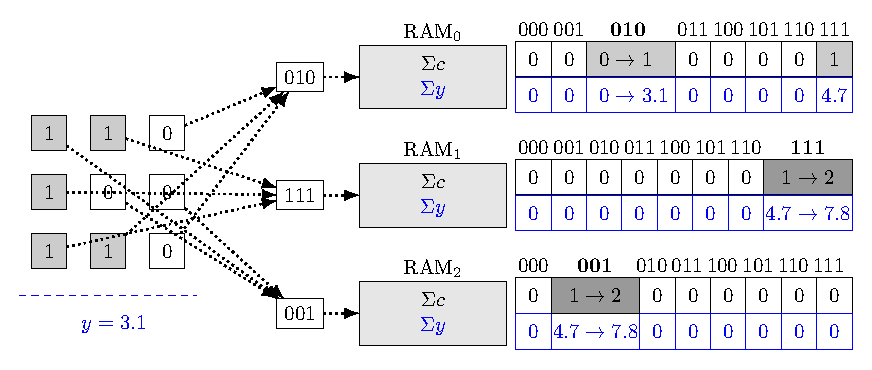
\includegraphics[width=0.75\textwidth]{fig_regwis2.pdf}
    \caption{Training ReW with the second sample}
    \label{fig_rew2}
\end{figure*}

Let $\hat{y}$ be the output estimate associated with a given input pattern $\chi$. Let $c_j$ and $y_j$ denote the positions ($\Sigma c$ and $\Sigma y$, respectively) addressed by this pattern in $\text{RAM}_j$, where $j = 0, \dots, N-1$. Computing $\hat{y}$ consists of applying an aggregation function, such as the arithmetic mean, harmonic mean, geometric mean, or median \citep{lusquino_extending_2020}.

ReW has an extension for handling dissimilar patterns called ClusRegression WiSARD (CReW), which makes it possible to identify structures in unknown or unlabeled data through clustering and enables unsupervised learning \citep{lusquino_extending_2020}. During training, new samples are presented to the discriminators already created and are learned by those whose response is sufficiently compatible with the presented pattern. If this classification criterion is not satisfied, a new discriminator is created, trained with the sample, and added to the list of discriminators. Additional parameters can be defined to limit the number of learned patterns and the total number of discriminators.

Because WNNs require binary inputs, real-valued data are first converted into binary representations. In thermometer encoding, each input value is encoded using $B$ bits, which determine the resolution of the representation. This encoding may take different variants, such as linear, Gaussian, and distributive thermometer encodings \citep{bacellar_distributive_2022}.


\section{Related Works}
\label{sec_related}


To map the literature on WNNs for regression, we searched the Web of Science (WoS) and Scopus databases without initially restricting the scope to time series. The search strategy combined terms related to WNNs (\textit{wisard}, \textit{WNN}$^*$, or \textit{n-tuple}, \textit{ram-based}, or \textit{weightless} \textit{neural network}$^*$) with \textit{regress}$^*$, \textit{forecast}$^*$, or \textit{predict}$^*$. The queries retrieved 36 records from WoS and 73 from Scopus, totaling 109 records.

Screening proceeded in two stages. First, duplicates and documents classified as letters or conference reviews were removed, leaving 62 records. Second, titles and abstracts were screened for relevance, excluding studies that did not use WNNs for regression. This process yielded 10 studies, which were grouped according to their contributions to regression methods, empirical applications, and the modeling of sequential data.

The first set of works establishes the transition from WNN classification to WNN regression. \citet{kolcz_ntuple_1996} introduce the $n$-tuple regressor as a nonparametric estimator, while \citet{kolcz_ntuple_2000} combine regression with decision trees, indicating that weightless structures can be integrated with other predictive mechanisms. \citet{lusquino_extending_2020} propose ReW and CReW and explore ensemble strategies involving these architectures. In a different direction, \citet{katopodis_functional_2022} present an $n$-tuple network with gradient optimization, aimed at regression and online learning in nonstationary scenarios. Together, these works show that WNNs can be adapted to numerical prediction, but they do not specifically address temporal representation as a central modeling problem.

A second group of studies evaluates ReW and CReW in applied regression settings, emphasizing the empirical competitiveness and computational efficiency of these architectures. \citet{lusquino_prediction_2019} employ ReW and CReW for palm oil production forecasting, obtaining competitive performance among more than 50 models. \citet{lusquino_extending_2020} evaluate WiSARD variants in real estate price prediction and motor impairment prediction in Parkinson's patients, reporting competitive results and a substantial reduction in training times. \citet{lusquino_aweightless_2020} use ReW and CReW in multimodal empathy modeling, highlighting the response speed of the architectures, although the results remain below the state of the art. These applications reinforce the potential of WNNs for regression, while also indicating that competitiveness depends on the domain, the representation adopted, and the reference methods considered.

The third group comprises works that use WNNs to represent or explore sequential data, but without fully centering the problem on direct time series forecasting. \citet{desouza_fast_2011} use an image-based WNN to forecast stock returns, obtaining performance comparable to that of a traditional ANN with significantly lower computational cost. \citet{alhassan_using_2011} develop a financial market forecasting system based on matching historical patterns, whose generalization ability is limited by dependence on literal matches. In turn, \citet{oliveira_fault_2017} employ WNNs for fault detection in time series, achieving high accuracies in two case studies. These works are important because they show that WNNs can process temporally ordered data, but their representations tend to treat temporal structure indirectly, either through image-like encodings, exact pattern matching, or detection-oriented formulations.

The works most directly related to time series forecasting with WNNs remain limited in scope and evaluation breadth. In an experiment presented by \citet{lusquino_extending_2020}, ReW and CReW are used to predict sea temperature from salinity, showing competitive performance and computational advantages. \citet{rocha_regression_2020} propose a ReW-based architecture for controlling STATCOM devices, using temporal windows formed by concatenating binary vectors and obtaining lower MSE and faster responses than the traditional controller. Although these studies are closer to the objective of this work, they still rely on comparatively simple temporal representations and do not provide a broad assessment across heterogeneous datasets and forecasting baselines.

Despite these contributions, the main gaps identified in the reviewed studies are concentrated in the use of simple representations of temporal dynamics \citep{desouza_fast_2011, alhassan_using_2011, lusquino_extending_2020, rocha_regression_2020, katopodis_functional_2022}, which restricts the capture of series dependencies and generalization capacity \citep{baby_cawnn_2026}. We also did not identify comprehensive evaluations with different datasets and systematic comparisons with classical and state-of-the-art methods, which limits understanding of their potential in diverse scenarios.


\section{ForeSight}
\label{sec_foresight}


This section presents ForeSight, a method designed to address the limitations identified in Section~\ref{sec_related}.
ForeSight integrates temporal embeddings with WNNs, such as ReW and CReW. The predictive problem addressed by the method consists in learning, from the transformed windows $w_i$ and their associated targets $x'_{i+s}$, a function capable of estimating the next transformed observation and then returning the prediction to the original domain. The temporal encoding stage is designed to represent dependencies in a latent space before the data are processed by the weightless network. Thus, the weightless network operates on inputs in which the temporal structure is implicitly preserved.

In addition, the use of embeddings seeks to mitigate limitations associated with the non-extrapolative nature of WNNs. Because the weightless network computes predictions from previously observed patterns, any instance that leads to an unseen memory position results in a \textit{don't know answer} \citep{lusquino_extending_2020}, reflecting the absence of knowledge for that context. This situation tends to be more frequent in time series, especially in the presence of nonstationarity and distribution shifts over time \citep{ogasawara_event_2025}. ForeSight therefore uses embeddings as a representation mechanism intended to improve the WNN's handling of previously unseen sequences.

The proposed method is illustrated in Figure~\ref{fig_method}. The workflow starts from an original time series $X$, which is subjected to preprocessing operations such as nonstationarity treatment \citep{salles_nonstationary_2019}, normalization \citep{han_data_2012}, and data augmentation \citep{iglesias_data_2023}. These transformations result in the modified series $X'$. In the evaluation protocol, these operations are controlled by the TSPredIT workflow and are treated as preprocessing steps or modeling hyperparameters when applicable.

\begin{figure*}[!ht]
    \centering
    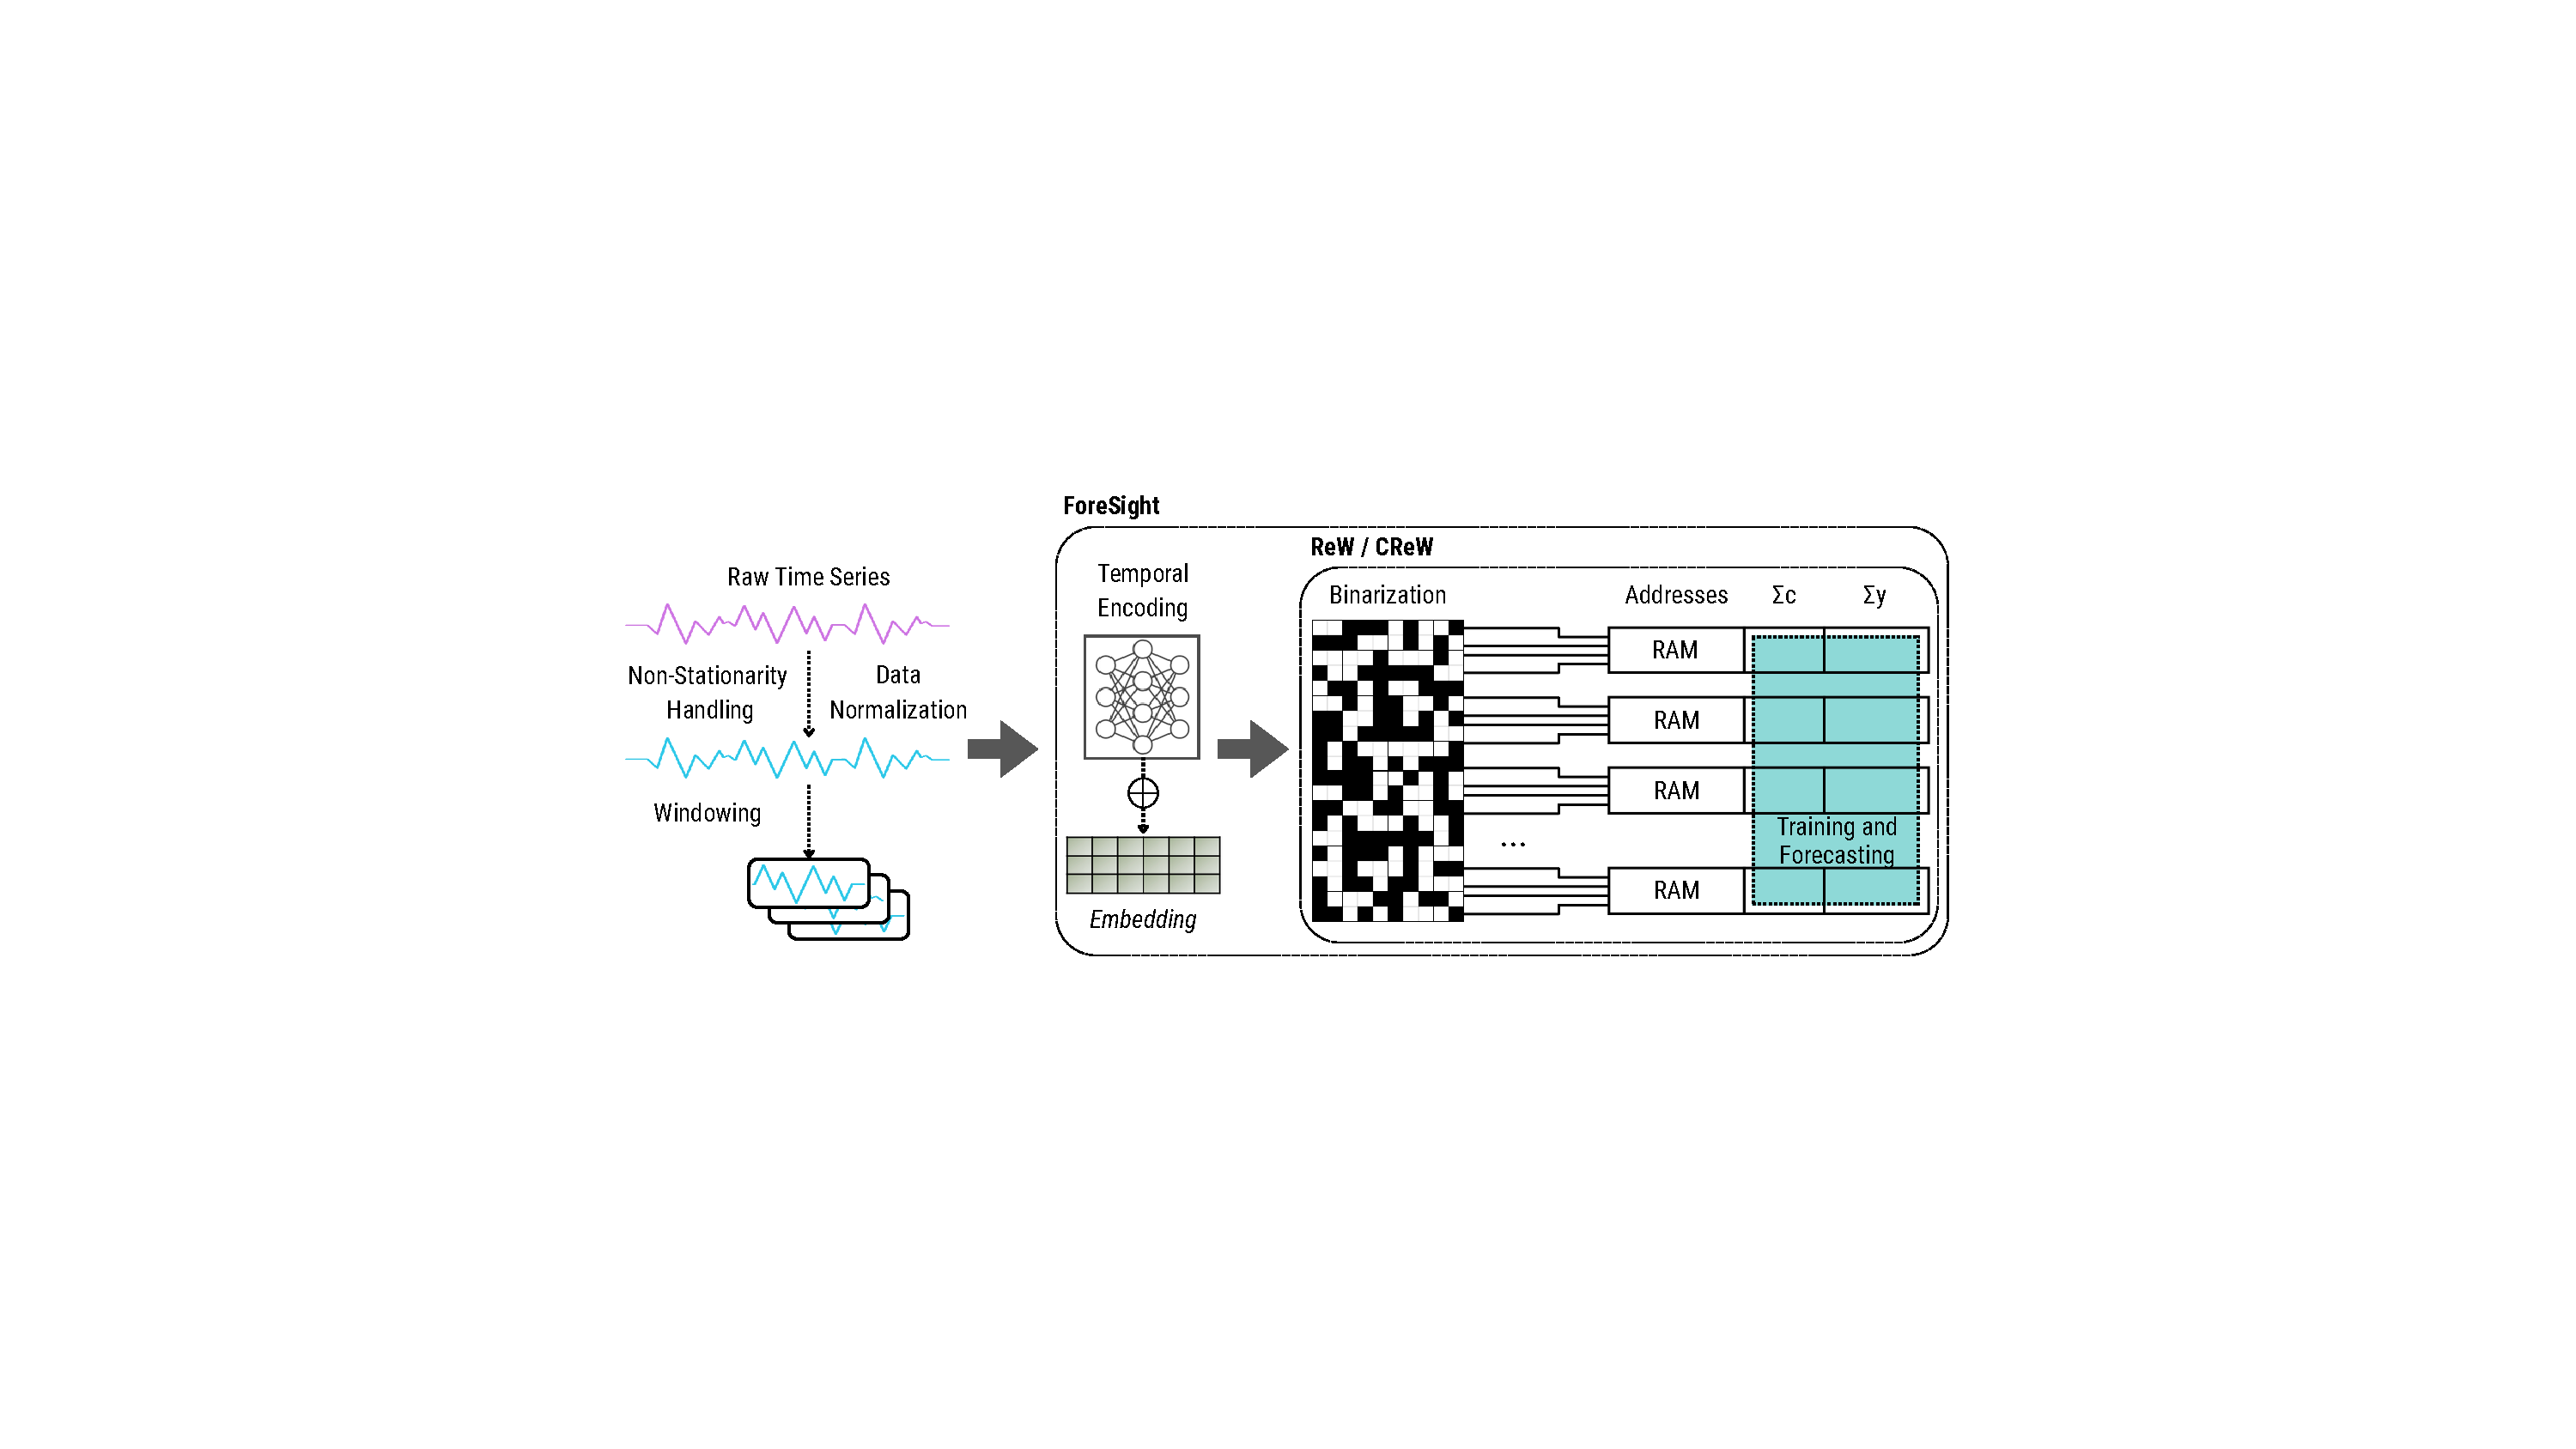
\includegraphics[width=0.95\textwidth]{fig_method.pdf}
    \caption{Time series forecasting with ForeSight}
    \label{fig_method}
\end{figure*}

Next, the SW procedure is applied to $X'$, converting the series into a set of pairs formed by windows of past observations and their corresponding following values. Let $W_{m \times s}$ contain the $m=|X'|-s$ supervised input windows, where row $w_i=\{x'_i,\dots,x'_{i+s-1}\}$ is associated with target $x'_{i+s}$ for $i=1,\dots,m$.

For each window $w_i$, a temporal encoding function $f$ is adopted to generate dense representations in a continuous $r$-dimensional space, that is, $f : w_i \mapsto \omega_i$, with $\omega_i \in \mathbb{R}^{1\times r}$. This stage projects subsequences into a latent space in which relevant patterns are preserved, providing a more expressive input basis for the WNN.

For the network to operate on these vectors, they must be converted into binary representations. Letting $B$ be the number of encoding bits, each vector $\omega_i$ is binarized by thermometer techniques to generate a retina $\chi_i$ of size $M = r \times B$. Although recent works on WNNs adopt Gaussian thermometer encoding \citep{susskind_weightless_2022, susskind_uleen_2023}, distributive thermometer encoding is less restrictive with respect to data distribution and the minimum size of the latent space dimension, favoring its application with different embedding techniques \citep{bacellar_distributive_2022}. Training occurs iteratively with the retinas $\chi_i$, associating each binary pattern with the observation $x'_{i+s}$ at the subsequent instant. The resulting prediction pipeline is summarized by Equation~\ref{eq_foresight_pred}, where $b(\cdot)$ denotes the binarization function and $g_{\theta}$ represents the trained WNN model, parameterized by the memory contents learned from the training retinas.

\begin{equation}
\label{eq_foresight_pred}
    \hat{x}'_{i+s} = g_{\theta}(\chi_i), \quad \chi_i = b(f(w_i))
\end{equation}

Values are stored in the memory positions addressed by the corresponding retinas. Thus, ForeSight learns from latent representations generated by the temporal encoder rather than directly from series windows.

Finally, inference follows the same procedure to access RAM contents, with the estimate $\hat{x}'_{i+s}$ passing through the inverse transformations of the initial stage and returning to the original domain. The flexible nature of ForeSight also allows alternative modeling of the original series, such as decomposition into trend, seasonality, and noise. The method can be applied independently to one or more components and the final prediction can be obtained by recomposition, enabling the dynamics of each component to be modeled separately \citep{hyndman_forecasting_2021}.

From a computational perspective, ForeSight preserves the linear complexity of WNNs with respect to the number of samples, which in this case corresponds to the $m$ processed windows. The overall complexity of the method depends on the temporal encoder used and can be expressed as $O\left(C_{\textit{emb}} + m\dfrac{rB}{n}\right)$, where $C_{\textit{emb}}$ represents the total cost of generating embeddings. This modular structure makes it possible to explore different representation techniques while keeping the WNN stage linearly dependent on the number of processed windows, balancing predictive performance and computational cost according to the application.


\section{Integration into TSPredIT}
\label{sec_framework}


The limitations identified in the reviewed studies motivate the development of an evaluation workflow to investigate ForeSight's performance in multiple scenarios. The method was implemented in Python 3.12 using the \texttt{wisardpkg} library \citep{lima_wisardpkg_2020} and integrated into the TSPredIT package. TSPredIT is an open-source R package for time series forecasting that integrates data preprocessing, lag selection, augmentation, normalization, and prediction. It supports statistical methods, traditional ML algorithms, and neural-network architectures, as well as multiple forecasting strategies and integrated tuning of input configurations and model hyperparameters, enabling systematic comparisons of forecasting pipelines.

This integration allows ForeSight to use TSPredIT operations beyond those considered in this research, including nonstationarity treatment, outlier removal, smoothing, and data augmentation. It also standardizes comparison with other methods and reproduction of the obtained results. Figure~\ref{fig_framework} presents an overview of the evaluation workflow, structured into three stages from top to bottom: time series selection and splitting; model training and tuning; and testing and results, with analysis and bookkeeping. Each stage consists of multiple steps, represented by boxes and letters. The model training and tuning stage comprises three distinct execution lanes, depending on the forecasting method. Within the ML lane, not all steps are required for every algorithm.   

\begin{figure*}[!ht]
    \centering
    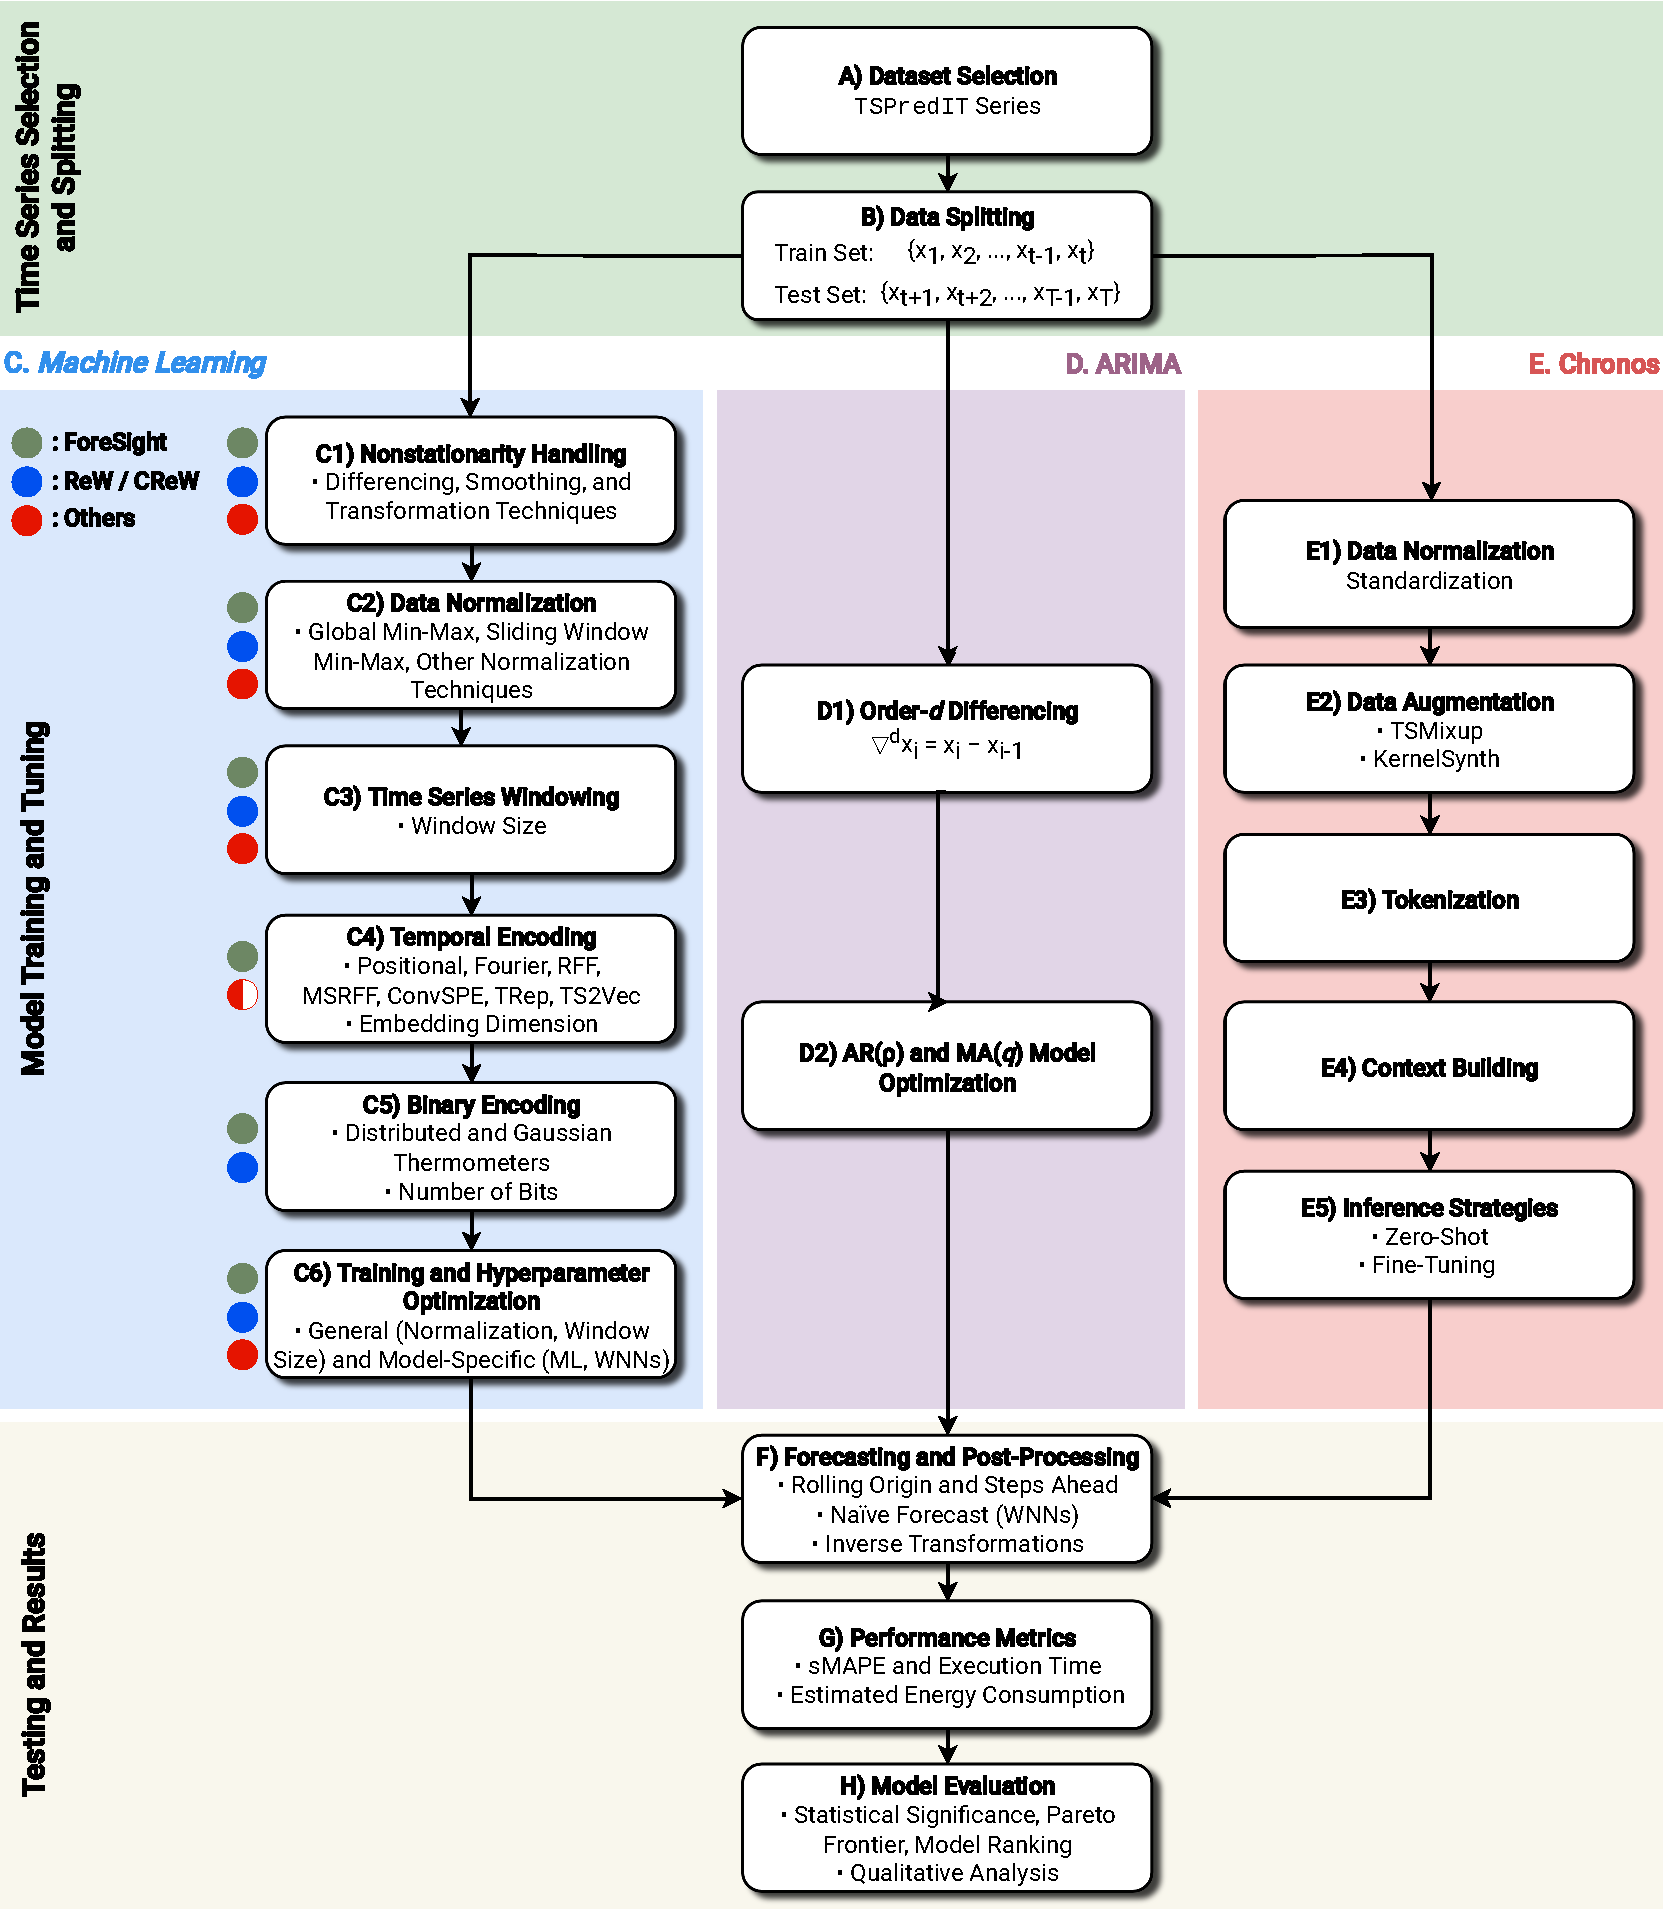
\includegraphics[width=0.95\textwidth]{fig_framework.pdf}
    \caption{ForeSight evaluation workflow in the TSPredIT package}
    \label{fig_framework}
\end{figure*}

Step~A corresponds to selecting the time series used in the experiments to evaluate ForeSight under distinct scenarios. Next, train-test partitioning is performed (Step~B). For this purpose, TSPredIT gathers time series from different applications and domains, in addition to providing predefined partitions for evaluation. Considering a series $X$ of size $T$ and cutoff point $t$, the training set is $\{x_1,\dots,x_t\}$, while observations $\{x_{t+1},\dots,x_T\}$ are used for testing. This split ensures evaluation on unseen data and enables computation of the metrics presented in Section~\ref{sec_background}.

For ML algorithms, Steps~C1--C3 correspond to the usual preprocessing operations \citep{anonymous_2023}. The techniques and parameters used, such as normalization strategies and SW size, become modeling hyperparameters. The same applies to the dimension $r$ of the latent space and to the temporal encoding technique used in ForeSight. Step~C4 considers different embedding generation techniques, including fixed encodings (PE, FE, RFF, and MSRFF) and learnable encodings (ConvSPE, TS2Vec, and TRep).

Step~C5 covers binarization and retina construction, employing thermometer encoding and varying the number $B$ of bits. This choice constitutes an additional modeling hyperparameter because it determines the granularity of discretization and, consequently, the degree of information loss inherent to the encoding process \citep{susskind_uleen_2023}. In ForeSight, binarization is applied after temporal encoding, so the retina is constructed from the latent representation rather than directly from the original window.

Models are trained in Step~C6, with hyperparameter optimization via grid search. Combinations of predefined values are exhaustively tested to identify the most suitable configuration for each algorithm. For this purpose, the training set is successively partitioned into training and validation subsets using time series cross-validation, preserving the temporal order of observations during model selection \citep{hyndman_forecasting_2021}. At the end, the configuration with the best average validation performance is selected and used to generate predictions on the test set. This procedure reduces the influence of a single data partition during optimization, minimizes the risk of overfitting, and makes comparison among methods more reliable.

The ARIMA operations are represented in Steps~D1--D2. First, parameter $d$ (differences) is defined to stabilize the mean and make the series stationary. Then, parameters $\rho$ and $q$ are guided by the autocorrelation and partial autocorrelation functions of the transformed series \citep{kontopoulou_areview_2023}. Starting from an initial ARIMA model, a systematic search is performed for other combinations capable of achieving better predictive performance, denoting the final configuration as $\text{ARIMA}(\rho^*,d^*,q^*)$ \citep{hyndman_automatic_2008}.

Chronos follows Steps~E1--E5. Initially, data standardization is applied. Then, the model applies synthetic sample generation techniques, such as TSMixup and KernelSynth \citep{ansari_chronos_2024}, to increase observation diversity and capture varied temporal structures. Finally, the transformed series are tokenized and the sequential context is built, enabling inference of the distribution over the next token(s) in the temporal flow, both in zero-shot mode and after fine-tuning.

Step~F consists of generating predictions on the test set using the rolling origin (RO) and steps ahead (SA) strategies \citep{hyndman_forecasting_2021}. In RO, models requiring fitting are fitted once and generate sequential one-step forecasts using each newly observed test value to update the input context, without refitting at each origin. In SA, the complete horizon is generated without observing intermediate test values; sliding-window methods therefore update their input recursively with previous predictions. For probabilistic models, such as Chronos, multiple inferences are performed, and the final result is obtained by aggregating these estimates, for example, by the mean or median. Predictions are converted back to the original domain of the series through the inverse transformations of the previous steps. In WNNs, outputs of the \textit{don't know answer} type are handled using the naïve forecast strategy \citep{hyndman_forecasting_2021}, which returns the last known observation as the prediction.

In Step~G, predictive quality is measured by a global version of sMAPE, computed over the entire dataset \citep{montero_principles_2021}. Let $\mathcal{S}$ be the time series that compose a given dataset and $\mathcal{T}(X)$ the indices corresponding to the test partition of series $X\in\mathcal{S}$. Thus, $\mathcal{O} = \{(X,t)\mid X\in\mathcal{S},\ t\in\mathcal{T}(X)\}$ represents all observations belonging to the test partition of the series in $\mathcal{S}$. For each $(X,t)\in\mathcal{O}$, let $x_t$ and $\hat{x}_t$ be, respectively, the observed value and the predicted value of series $X$ at instant $t$. The calculation of global sMAPE for all series in $\mathcal{S}$, denoted by $\mathrm{sMAPE}_{\mathcal{S}}$, is expressed by Equation~\ref{eq_smape_global}:

\begin{equation}
\label{eq_smape_global}
\mathrm{sMAPE}_{\mathcal{S}} = \frac{100}{|\mathcal{O}|} \sum_{(X,t)\, \in\, \mathcal{O}} \frac{2\,|\hat{x}_{t}-x_{t}|}{|\hat{x}_{t}|+|x_{t}|}
\end{equation}

This procedure is useful when there are no substantial differences among the sizes of the sets $\mathcal{T}(X)$ or when the same weight should be assigned to each observation in $\mathcal{O}$. Aggregating all predictions into a single metric provides an evaluation of model performance over the set of series and facilitates direct comparison between different datasets and predictive methods. In addition to sMAPE$_\mathcal{S}$, runtimes are also recorded for relative efficiency analysis, as well as an estimate of energy consumption \citep{shahid_improving_2021}, based on processing time, utilization rate, and the power of the processor used in the experiment. The estimated energy consumption $E$ is computed according to Equation~\ref{eq_energy}, where $t_{\textit{run}}$ is the runtime, $\eta$ is the utilization rate, and $\Phi$ is the processor power.

\begin{equation}
\label{eq_energy}
E = t_{\textit{run}} \cdot \eta \cdot \Phi
\end{equation}

Finally, Step~H systematically documents the obtained results. This stage includes statistical significance tests of performance \citep{montgomery_applied_2011}, ranking of methods based on $\mathrm{sMAPE}_{\mathcal{S}}$ \citep{koning_them3_2005, makridakis_m5_2022}, and Pareto frontier analysis \citep{yang_multi_2014}, which makes it possible to assess the trade-off between predictive quality and computational efficiency. A qualitative analysis based on time series characteristics is also conducted \citep{lubba_catch22_2019}, using dimensionality reduction and clustering \citep{han_data_2012} to understand under which data properties the proposed method is most effective.


\section{Experimental Evaluation}
\label{sec_experiments}

This section compares ForeSight with classical and selected state-of-the-art methods for time series forecasting across several application domains and analytical perspectives. The results compare predictive performance and computational efficiency, while a qualitative analysis investigates how temporal characteristics relate to the effectiveness of ForeSight across different groups of time series.

\subsection{Evaluation Protocol}
\label{sec_protocol}

The data from TSPredIT contain hundreds of time series from diverse domains in a unified and structured format, facilitating the development, reproducibility, and comparative evaluation of predictive methods. The datasets include socioeconomic and environmental indicators made available through FAOSTAT \citep{fao_faostat_2024}, as well as series from the M1, M3, and M4 international forecasting competitions \citep{makridakis_accuracy_1982, makridakis_m3_2000, makridakis_m4_2020}. Table~\ref{tab_datasets} presents a summary of the datasets used, covering description, size, and partitioning.

\begin{table*}[!ht]
\centering
\caption{Experimental datasets}
\small{
\begin{tabular}{p{3.5cm}p{7.5cm}>{\centering\arraybackslash}m{2.0cm}>{\centering\arraybackslash}m{2.0cm}}
\hline
\shortstack{\textbf{Dataset}} & \textbf{Description} & \textbf{Observations} & \shortstack{\rule{0pt}{2.5ex}\textbf{Test}\\\textbf{Observations}} \\
\hline
Bioenergy (Consumption) & Annual biofuel consumption in terajoules & 33 & 5 \\
Bioenergy (Production) & Annual biofuel production in terajoules & 33 & 5 \\
Emissions ($\text{CH}_4$) & Total methane ($\text{CH}_4$) emissions per year & 61 & 5 \\
Emissions ($\text{CO}_2$) & Total carbon dioxide ($\text{CO}_2$) emissions per year & 32 & 5 \\
Emissions ($\text{N}_2\text{O}$) & Total nitrous oxide ($\text{N}_2\text{O}$) emissions per year & 61 & 5 \\
Fertilizers ($\text{K}_2\text{O}$) & Total potassium ($\text{K}_2\text{O}$) in annual fertilizer production & 62 & 5 \\
Fertilizers (N) & Total nitrogen (N) in annual fertilizer production & 62 & 5 \\
Fertilizers ($\text{P}_2\text{O}_5$) & Total phosphorus ($\text{P}_2\text{O}_5$) in annual fertilizer production & 62 & 5 \\
Inflation (Food) & Annual consumer price index for food & 26 & 5 \\
Inflation (General) & Annual consumer price index for goods and services & 26 & 5 \\
Climate Change & Annual surface temperature variation in $^\circ$C & 63 & 5 \\
Pesticides & Total pesticides used in agriculture per year & 33 & 5 \\
GDP & GDP (gross domestic product) in dollars per year & 54 & 5 \\
M1 (Monthly) & Monthly series from the M1 competition & 48 to 150 & 18 \\
M1 (Quarterly) & Quarterly series from the M1 competition & 18 to 114 & 8 \\
M1 (Yearly) & Yearly series from the M1 competition & 15 to 58 & 6 \\
M3 (Monthly) & Monthly series from the M3 competition & 66 to 144 & 18 \\
M3 (Quarterly) & Quarterly series from the M3 competition & 24 to 72 & 8 \\
M3 (Unspecified) & Series with unspecified frequency from the M3 competition & 71 to 104 & 8 \\
M3 (Yearly) & Yearly series from the M3 competition & 20 to 47 & 6 \\
M4 (Daily) & Daily series from the M4 competition & 107 to 9,933 & 14 \\
M4 (Hourly) & Hourly series from the M4 competition & 748 to 1,008 & 48 \\
M4 (Monthly) & Monthly series from the M4 competition & 60 to 2,812 & 18 \\
M4 (Quarterly) & Quarterly series from the M4 competition & 28 to 874 & 8 \\
M4 (Weekly) & Weekly series from the M4 competition & 93 to 2,610 & 13 \\
M4 (Yearly) & Yearly series from the M4 competition & 19 to 841 & 6 \\
\hline
\end{tabular}
}
\label{tab_datasets}
\end{table*}

To characterize the heterogeneity of temporal dynamics and investigate the performance of predictive models in groups with similar properties, a feature-based clustering step was performed. This procedure represents each series by a set of characteristics covering statistical moments, dependency patterns, and spectral properties, making it particularly suitable for datasets from different domains, structures, and lengths \citep{fulcher_highly_2014}. For feature extraction, \texttt{catch22} was used \citep{lubba_catch22_2019}, which provides a compact set of 22 canonical features selected from a broader context of temporal data measures. After extraction, the metrics were standardized and subjected to dimensionality reduction via principal component analysis (PCA), making it possible to identify those with the greatest contribution to the variability represented by the components.

Based on this characterization, the series are grouped according to the similarity of their properties using the $K$-Means algorithm. The number of groups $K$ was determined by analyzing the silhouette coefficient, targeting values above $0.5$ \citep{han_data_2012}. Thus, the adopted configuration sought to obtain sufficiently distinct groups to compare predictive methods according to the predominant characteristics of each set.

Hyperparameters were defined empirically, with adjustments made according to the particularities of each dataset. Window size $s$ for the UN series followed values in $\{6, 8\}$. In the forecasting competition sets, windows were configured according to periodicity: $\{6, 8\}$ for yearly series, $\{8, 12\}$ for quarterly, monthly, or unspecified series, and $\{14, 28\}$ for weekly, daily, or hourly series. In all cases, the complete sequence was used as model input, without subsampling observations.

For embedding generation, ForeSight incorporated all techniques presented in Section~\ref{sec_embeds}, adopting values of $r$ in $\{16, 32, 64, 128, 256\}$. This variation makes it possible to investigate the impact of latent space dimensionality, seeking the best balance between representation capacity, predictive performance, and computational efficiency. The method was implemented with ReW and CReW, the latter limited to $10$ discriminators and $10 \times m$ samples per discriminator.

Table~\ref{tab_hiperparametros} presents the remaining hyperparameter configurations of the ML methods, where the notation (\mbox{0.0, 1.0, 0.1}), for example, indicates variation from 0.0 to 1.0 in increments of 0.1. To facilitate reading, the table uses parameter names instead of the mathematical notation adopted throughout the text. The values presented correspond to the search space used during model optimization, while parameters not listed in the table followed the defaults defined in TSPredIT and in the underlying libraries.

\begin{table}[ht]
\centering
\caption{Configuration of ML methods in the TSPredIT package}
\label{tab_hiperparametros}
\small
\setlength{\tabcolsep}{3pt}
\begin{tabularx}{\columnwidth}{@{}
>{\centering\arraybackslash}p{1.8cm}
X
@{}}
\hline
\textbf{Method} & \multicolumn{1}{c}{\textbf{Hyperparameters}} \\
\hline
\multirow[c]{2}{*}{\shortstack{ForeSight / \\ReW / CReW}}
& bits = \{8, 16, 32\} \\
& RAM size = \{4, 8, 16\} \\
\hline
\multirow{2}{*}{\shortstack{Conv1D\\LSTM}}
& learning rate = (0.01, 0.05, 0.01) \\
& epochs = $10^3$ \\
\hline
\multirow{3}{*}{ELM}
& neurons in the hidden layer = (1, 10, 1) \\
& activation function = \{\textit{``sig'', ``relu'', ``purelin''}\} \\
\hline
\multirow{2}{*}{$k$NN}
& $k$ = (3, 8, 1) \\
& distance metric = \textit{``euclidean''} \\
\hline
\multirow{3}{*}{MLP}
& neurons in hidden layers = (1, 10, 1) \\
& decay = (0.0, 1.0, 0.1) \\
& maximum iterations = $10^3$ \\
\hline
\multirow{2}{*}{RFR}
& number of trees = (10, 100, 20) \\
& terminal node size = (1, 10, 1) \\
\hline
\multirow{3}{*}{SVR}
& kernel = \{\textit{``radial'', ``linear'', ``sigmoid''}\} \\
& tolerance = (0.0, 1.0, 0.2) \\
& violation cost = (10, 100, 20) \\
\hline
\end{tabularx}
\end{table}

Regarding the other benchmark methods, the ARIMA implementation used the \texttt{auto-ARIMA} function \citep{hyndman_automatic_2008} to automatically adjust and calibrate parameters $(\rho^*, d^*, q^*)$. For Chronos, we employed the tiny version, with 256-dimensional tokens. The model generated $10^3$ independent inferences in zero-shot mode, using the mean as the final estimate.

The experiments followed the RO and SA strategies, analyzing the performance of the methods across different forecasting horizons and under varied generalization conditions. We repeated each experimental scenario five times to assess result variability and prediction stability. In each run, $\mathrm{sMAPE}$ and total processing time per series were collected. All tests were performed on a server with an Intel Xeon W3-2423 processor, equipped with 16 threads operating at 4.20~GHz and 512~GB of RAM. We estimated energy consumption in joules using Equation~\ref{eq_energy}, complementing computational cost information with energy-efficiency measures. The source code and configurations used to run the experiments are available in an accompanying repository\footnote{Repository URL withheld for double-anonymized review.}.

\subsection{Results and Discussion}
\label{sec_results}

Figure~\ref{fig_rank} transforms the errors measured by sMAPE at the series level into an average ranking capable of systematically ordering the methods across RO and SA predictions. The blue band represents the 95\% confidence interval associated with the configuration with the best ranking, while the configurations highlighted in red have some overlap with this interval. In both scenarios, ForeSight with MSRFF achieves the best ranking, followed by MLP and ARIMA, whereas ReW and CReW occupy the last positions. These results highlight the contribution of embedding-based representations to the predictive performance of WNNs.

\begin{figure*}[!ht]
    \centering
    \begin{subfigure}[b]{0.49\textwidth}
        \centering
        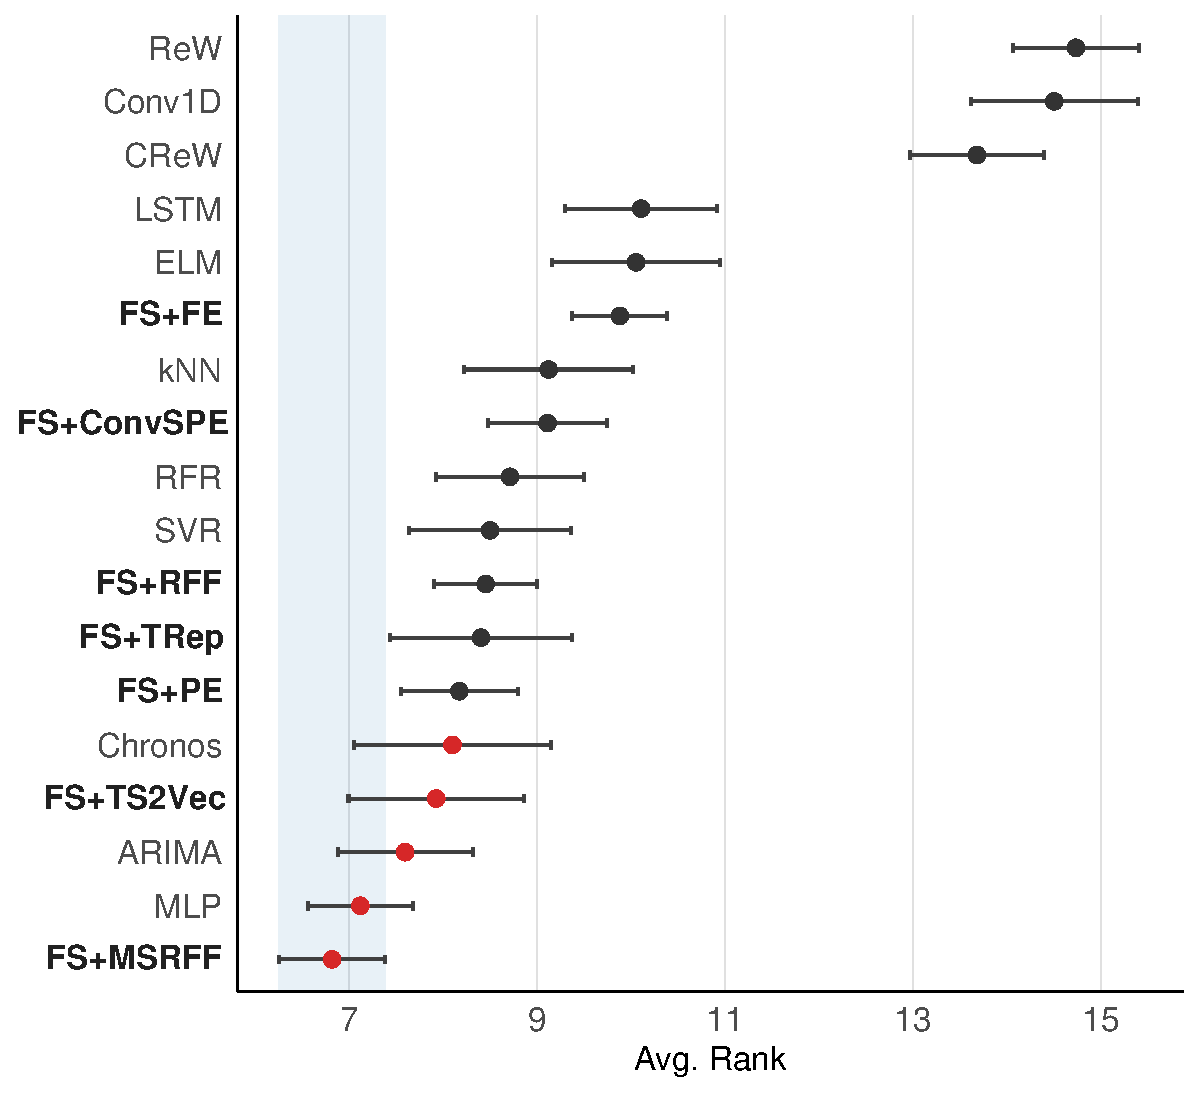
\includegraphics[width=\textwidth]{fig_rank_ro.pdf}
        \phantomcaption
        \label{fig_rank_ro}
    \end{subfigure}
    \hfill
    \begin{subfigure}[b]{0.49\textwidth}
        \centering
        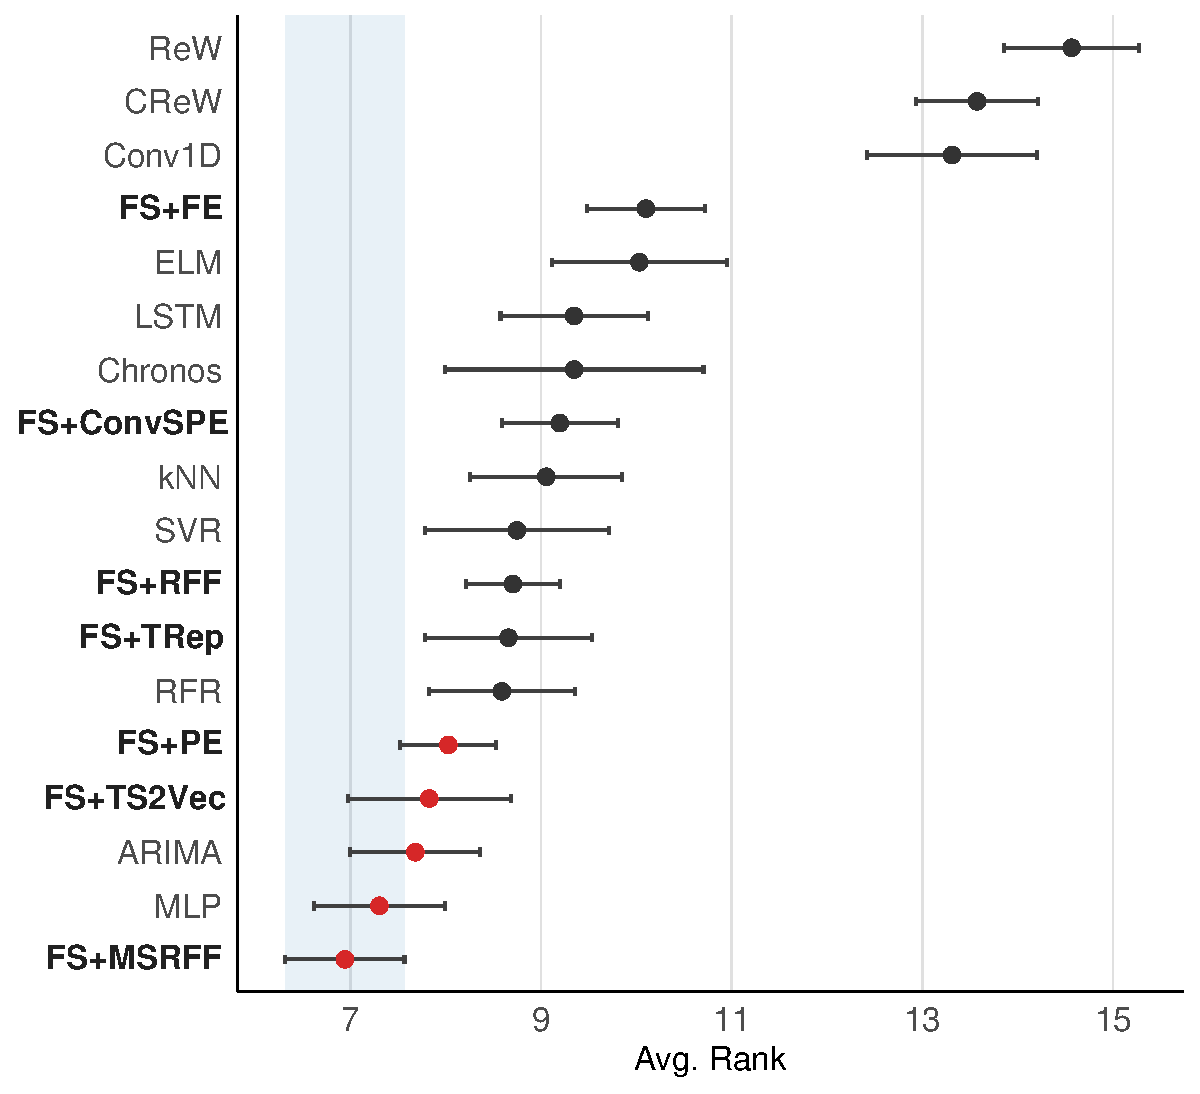
\includegraphics[width=\textwidth]{fig_rank_sa.pdf}
        \phantomcaption
        \label{fig_rank_sa}
    \end{subfigure}
    \vspace{-0.5cm}
    \caption{Ranking of predictive methods in the rolling origin (left) and steps ahead (right) scenarios.}
    \label{fig_rank}
\end{figure*}

To analyze how latent space size affects ForeSight's computational cost, we conducted a sensitivity analysis of the method combined with each temporal encoding technique, using vectors with $\{16, 32, 64, 128, 256\}$ dimensions. Figure~\ref{fig_time} shows the impact of this variation on the mean total runtime, including training and inference. Because one of WNNs' main characteristics is computational efficiency \citep{lusquino_extending_2020, susskind_weightless_2022}, this analysis verifies how the additional cost scales with $r$ for each encoding technique.

The runtime analysis shows that the TS2Vec- and TRep-based ForeSight variants have higher computational costs even at low embedding dimensions. In contrast, the fixed-encoding variants and ConvSPE have runtime values close to ReW and CReW at 16 dimensions, while processing-time differences become noticeable from 64 dimensions onward. Nevertheless, these variants remain faster than computationally efficient methods, such as ARIMA and $k$NN, even at higher embedding dimensions.

\begin{figure*}[!ht]
    \vspace{0.5cm}
    \centering
    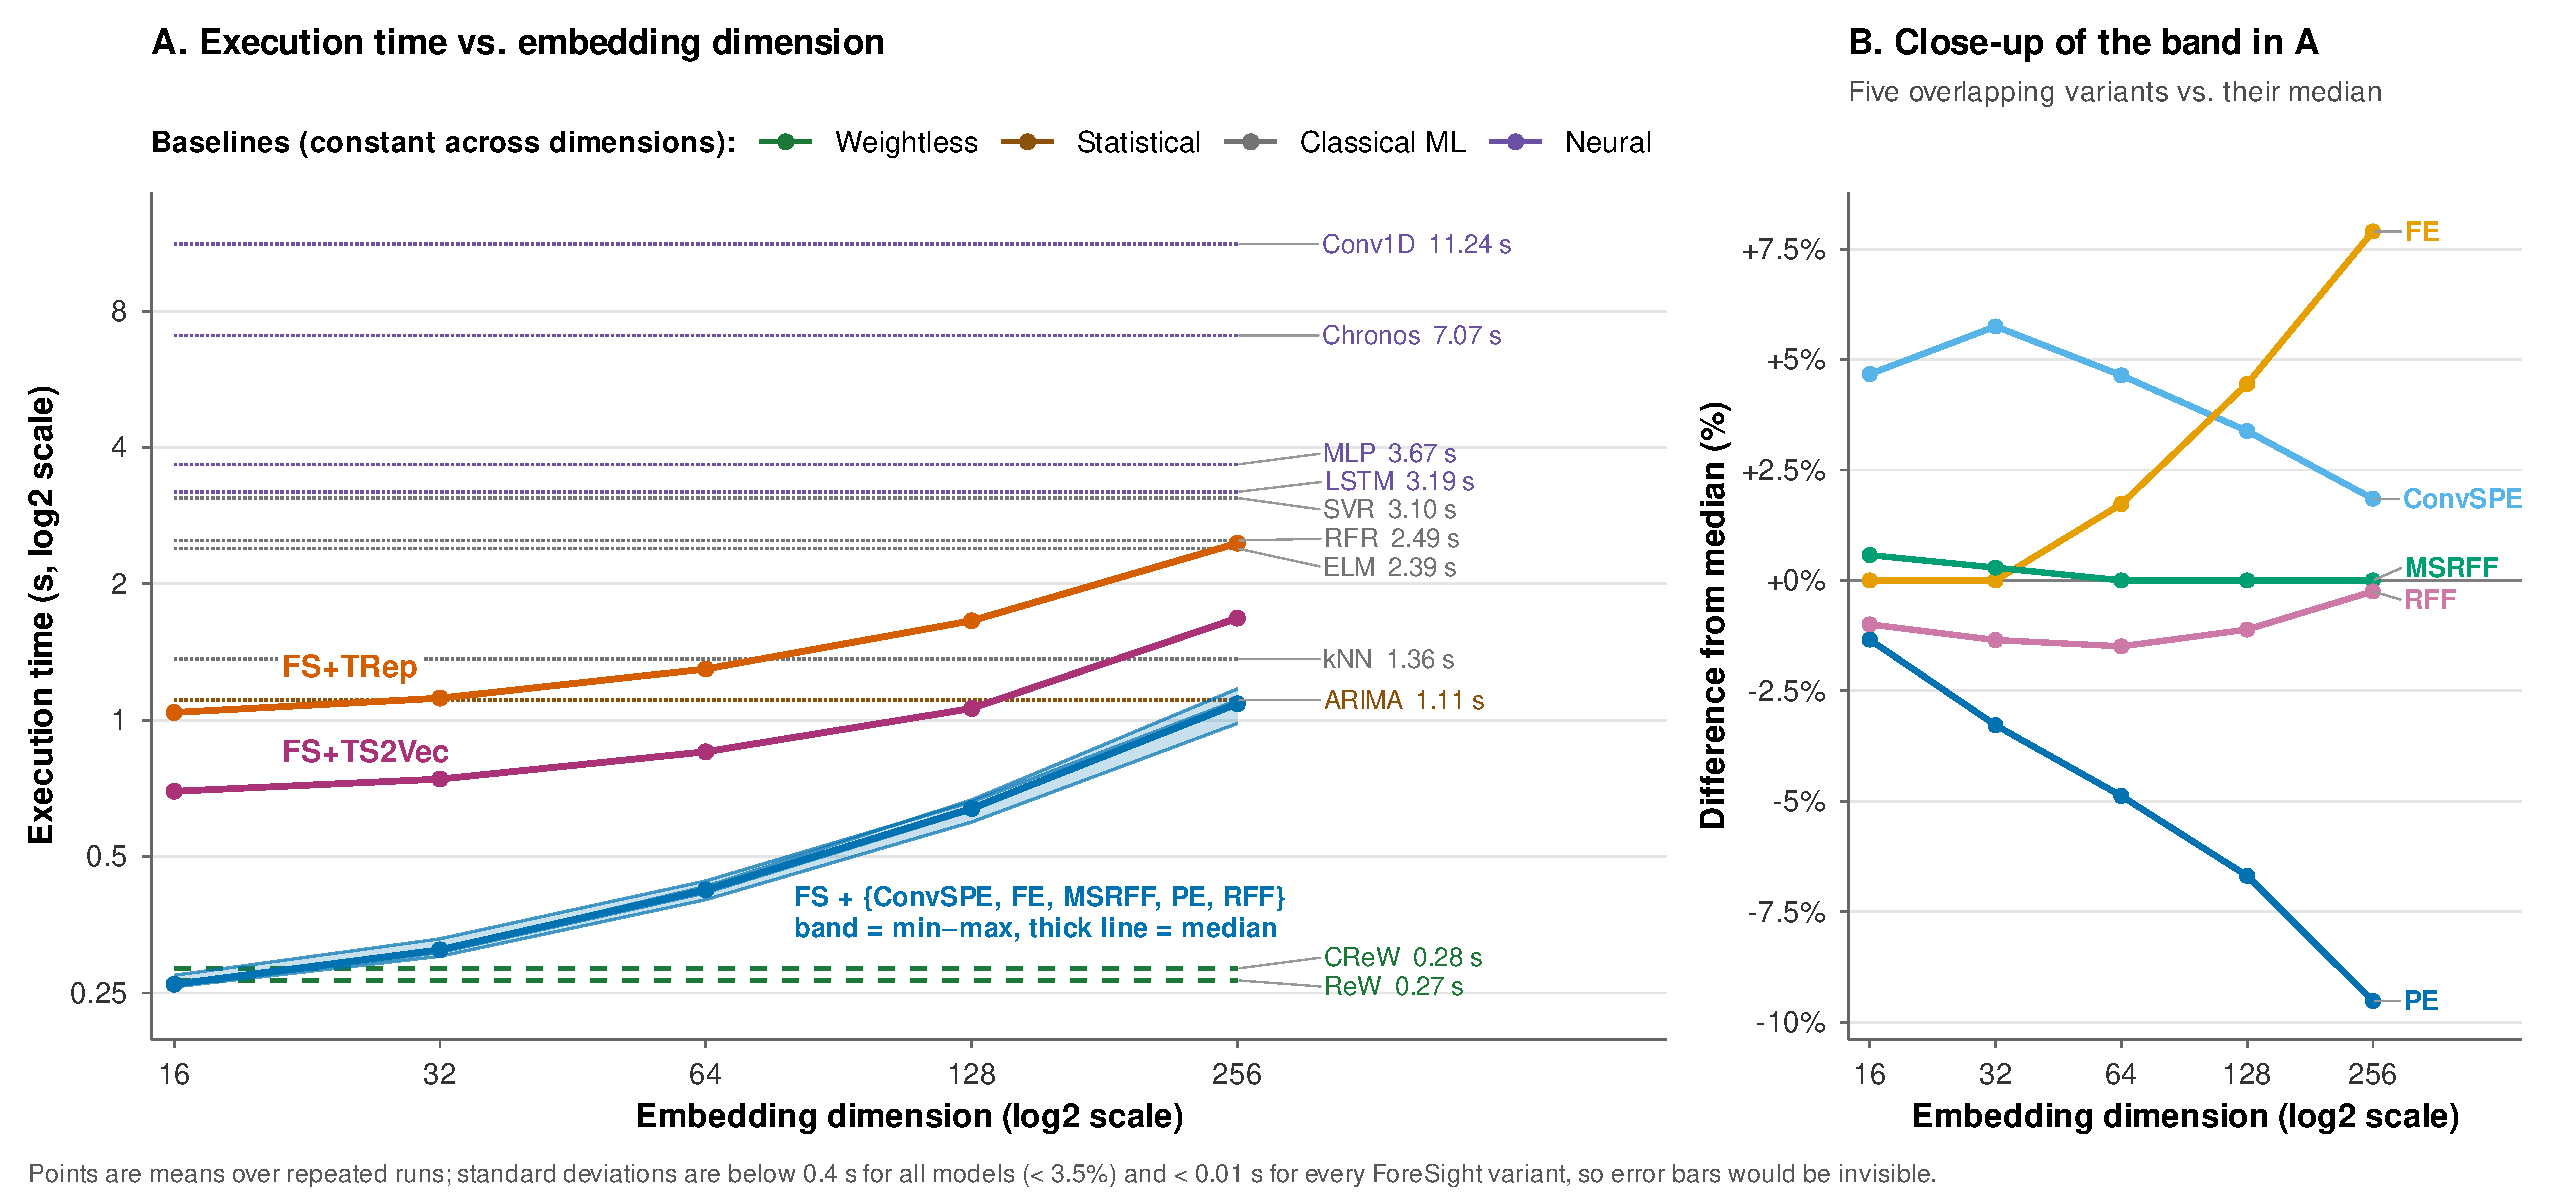
\includegraphics[width=0.95\textwidth]{fig_time.pdf}
    \caption{Variation in total processing time as a function of embedding dimensionality}
    \label{fig_time}
\end{figure*}

Figure~\ref{fig_pareto} relates the sMAPE calculated according to Equation~\ref{eq_smape_global} to the estimated average energy consumption per series, expressed in joules ($\mathrm{J}$), treating both as objectives to be minimized. The dashed line delimits the Pareto frontier, composed of nondominated solutions that cannot be outperformed simultaneously in both criteria. ReW and CReW exhibit the lowest energy consumption, while Chronos achieves the lowest sMAPE under RO and MLP under SA. In both scenarios, ForeSight with MSRFF lies on the Pareto frontier, offering a favorable trade-off between predictive performance and energy consumption.

\begin{figure*}[!htbp]
    \centering
    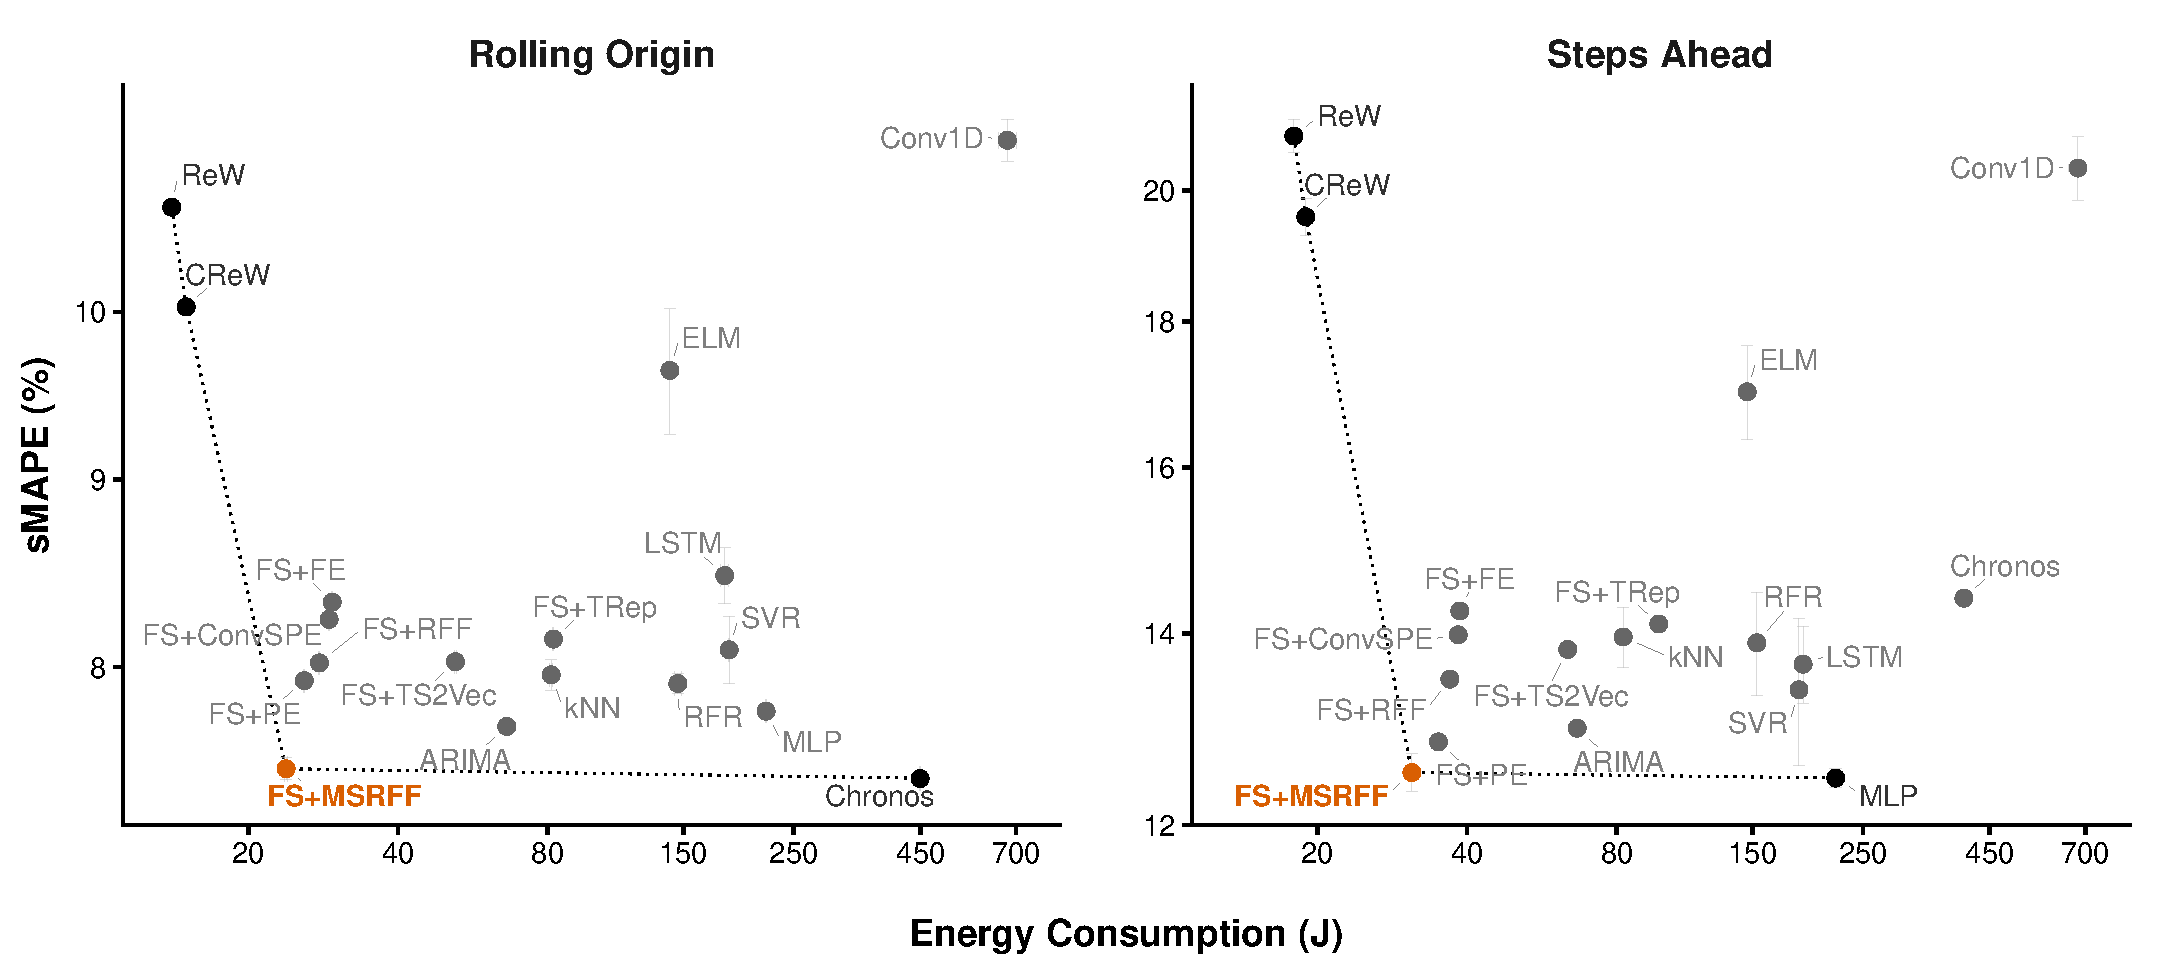
\includegraphics[width=0.95\textwidth]{fig_pareto.pdf}
    \caption{Pareto frontier between predictive performance and energy consumption}
    \label{fig_pareto}
\end{figure*}

These results address \textit{RQ1} by showing that ForeSight achieves competitive average rankings across heterogeneous series and maintains substantially lower runtimes than more computationally demanding alternatives. They address \textit{RQ2} by showing that the temporal encoding technique affects predictive performance, while increasing the latent dimension raises computational cost. Fixed encodings remain more efficient than the learned alternatives, and MSRFF provides the most favorable accuracy--efficiency trade-off among the evaluated ForeSight variants. \textit{RQ3} is examined next through the feature-based analysis of series properties.

Applying the characterization procedure described in Section~\ref{sec_protocol}, six features showed the greatest individual contribution and were used in the clustering operation.
Overall, these characteristics capture aspects related to oscillation (sign change rate and dominant oscillation frequency), linear temporal dependence (lag-1 linear autocorrelation, lag-2 linear autocorrelation, and overall linear dependence), and spectral complexity \citep{lubba_catch22_2019}. In other words, the clusters group series that share a similar temporal signature, distinguishing, on the one hand, more regular, persistent dynamics and, on the other, more oscillatory, complex behavior. This characterization makes the qualitative analysis more interpretable by allowing series properties to be related to the behavior of forecasting methods.

The first cluster comprises 168 series (64.6\%) with well-defined behavior and a more regular temporal signature. This structure tends to favor pattern identification and reuse, facilitating the forecasting task. Figure~\ref{fig_cluster_0} helps visually interpret these characteristics. In the first row, a synthetically generated series is shown to reproduce the properties of the group, along with its corresponding Fourier transform and the distribution of embeddings generated with MSRFF. In the second row, the same elements are presented for the series \texttt{biocons\_brazil}, selected as a representative example of the cluster from the Bioenergy (Consumption) dataset. Thus, the columns allow observation, respectively, of the behavior of observations in the time domain, their frequency composition, and the organization of subsequences in latent space.

Both the synthetic series and the example series present relatively smooth variations, with energy concentration at low frequencies in their respective transforms. Regarding the embeddings, the observations form organized and relatively continuous structures, with regions of higher point concentration. This suggests that, for this group, the latent representation preserves a clearer organization of subsequences, keeping those with similar temporal behaviors close together and contributing to the association of similar temporal states by predictive methods.

\begin{figure*}[!ht]
    \vspace{0.5cm}
    \centering
    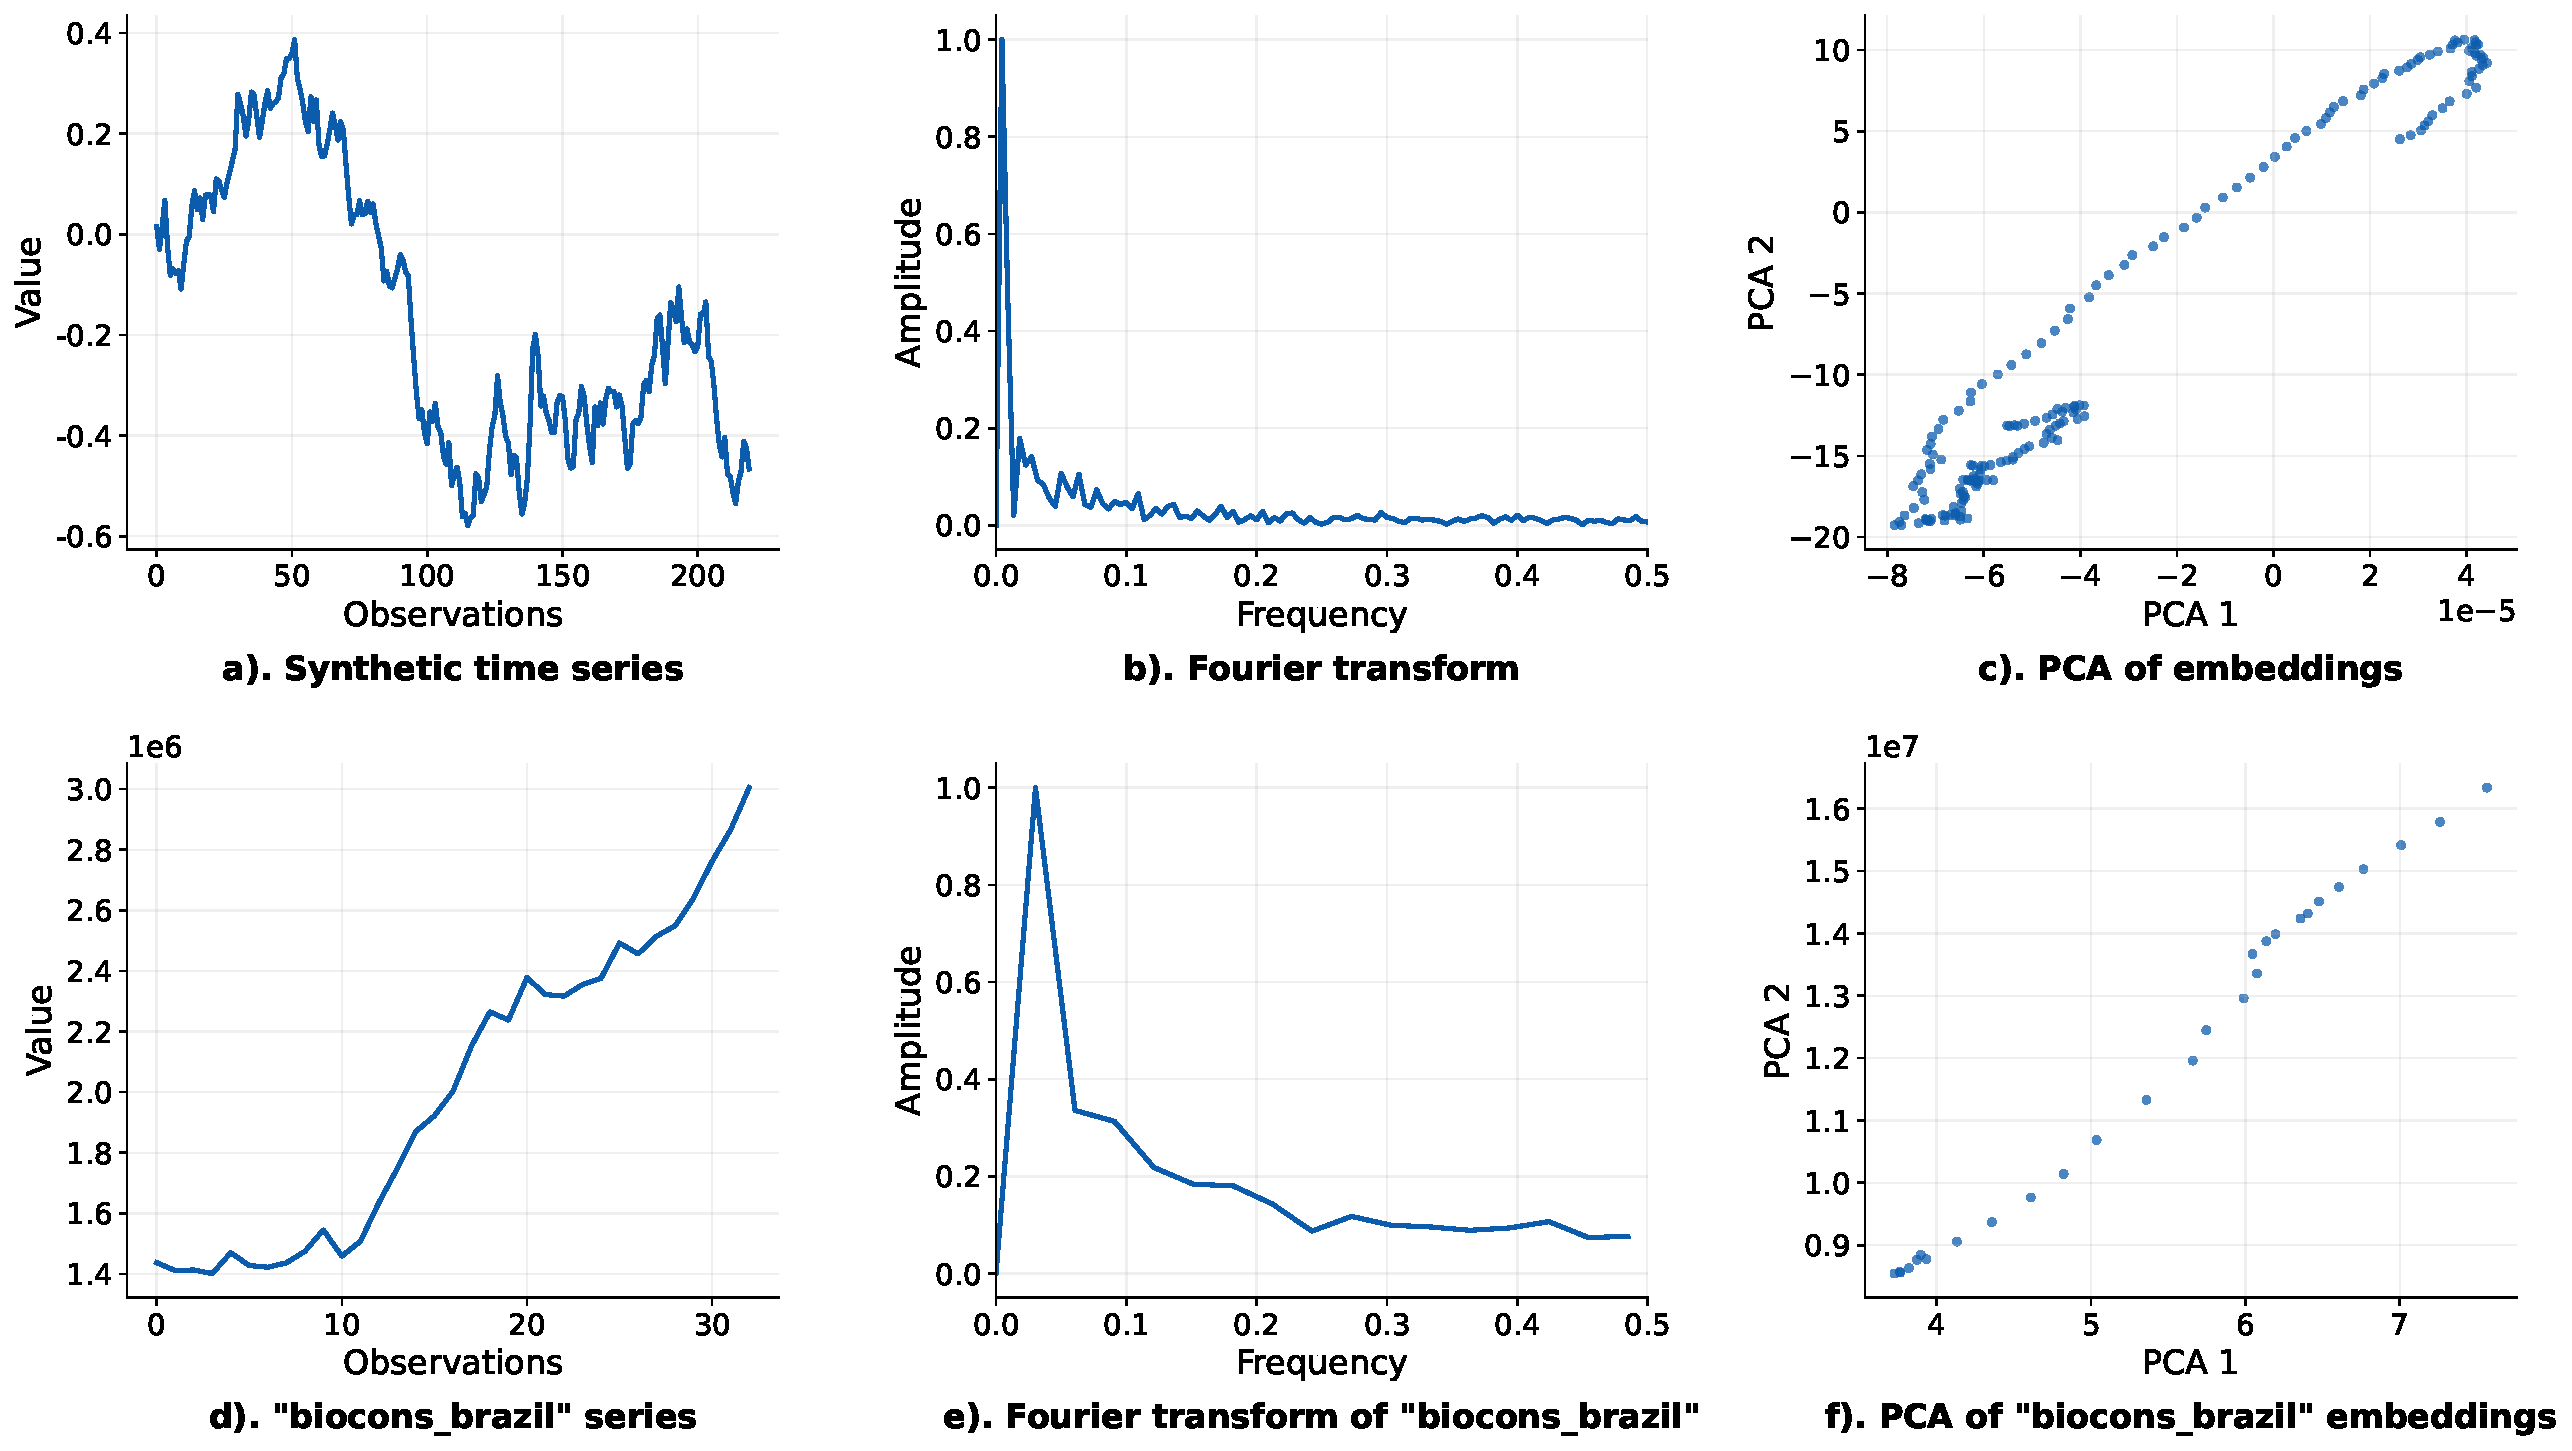
\includegraphics[width=0.95\textwidth]{fig_cluster_0.pdf}
    \caption{Characterization of series with more regular temporal behavior}
    \label{fig_cluster_0}
\end{figure*}

The second cluster contains 92 series (35.4\%) and exhibits distinct temporal behavior, as shown in Figure~\ref{fig_cluster_1}. The series \texttt{biocons\_canada}, also from the Bioenergy (Consumption) dataset, was selected as a representative example. Overall, the sequences are characterized by faster oscillations and greater irregularity, presenting multiple peaks and making the forecasting task more challenging for all methods. The transforms show amplitude distributed across different frequency components, while the embeddings occupy a more dispersed, heterogeneous region in latent space. This arrangement indicates less recurrence of similar temporal states, hindering the WNN's reuse of previously observed representations and, consequently, limiting the gains temporal encoding provides in generating ForeSight estimates.

\begin{figure*}[!ht]
    \vspace{0.5cm}
    \centering
    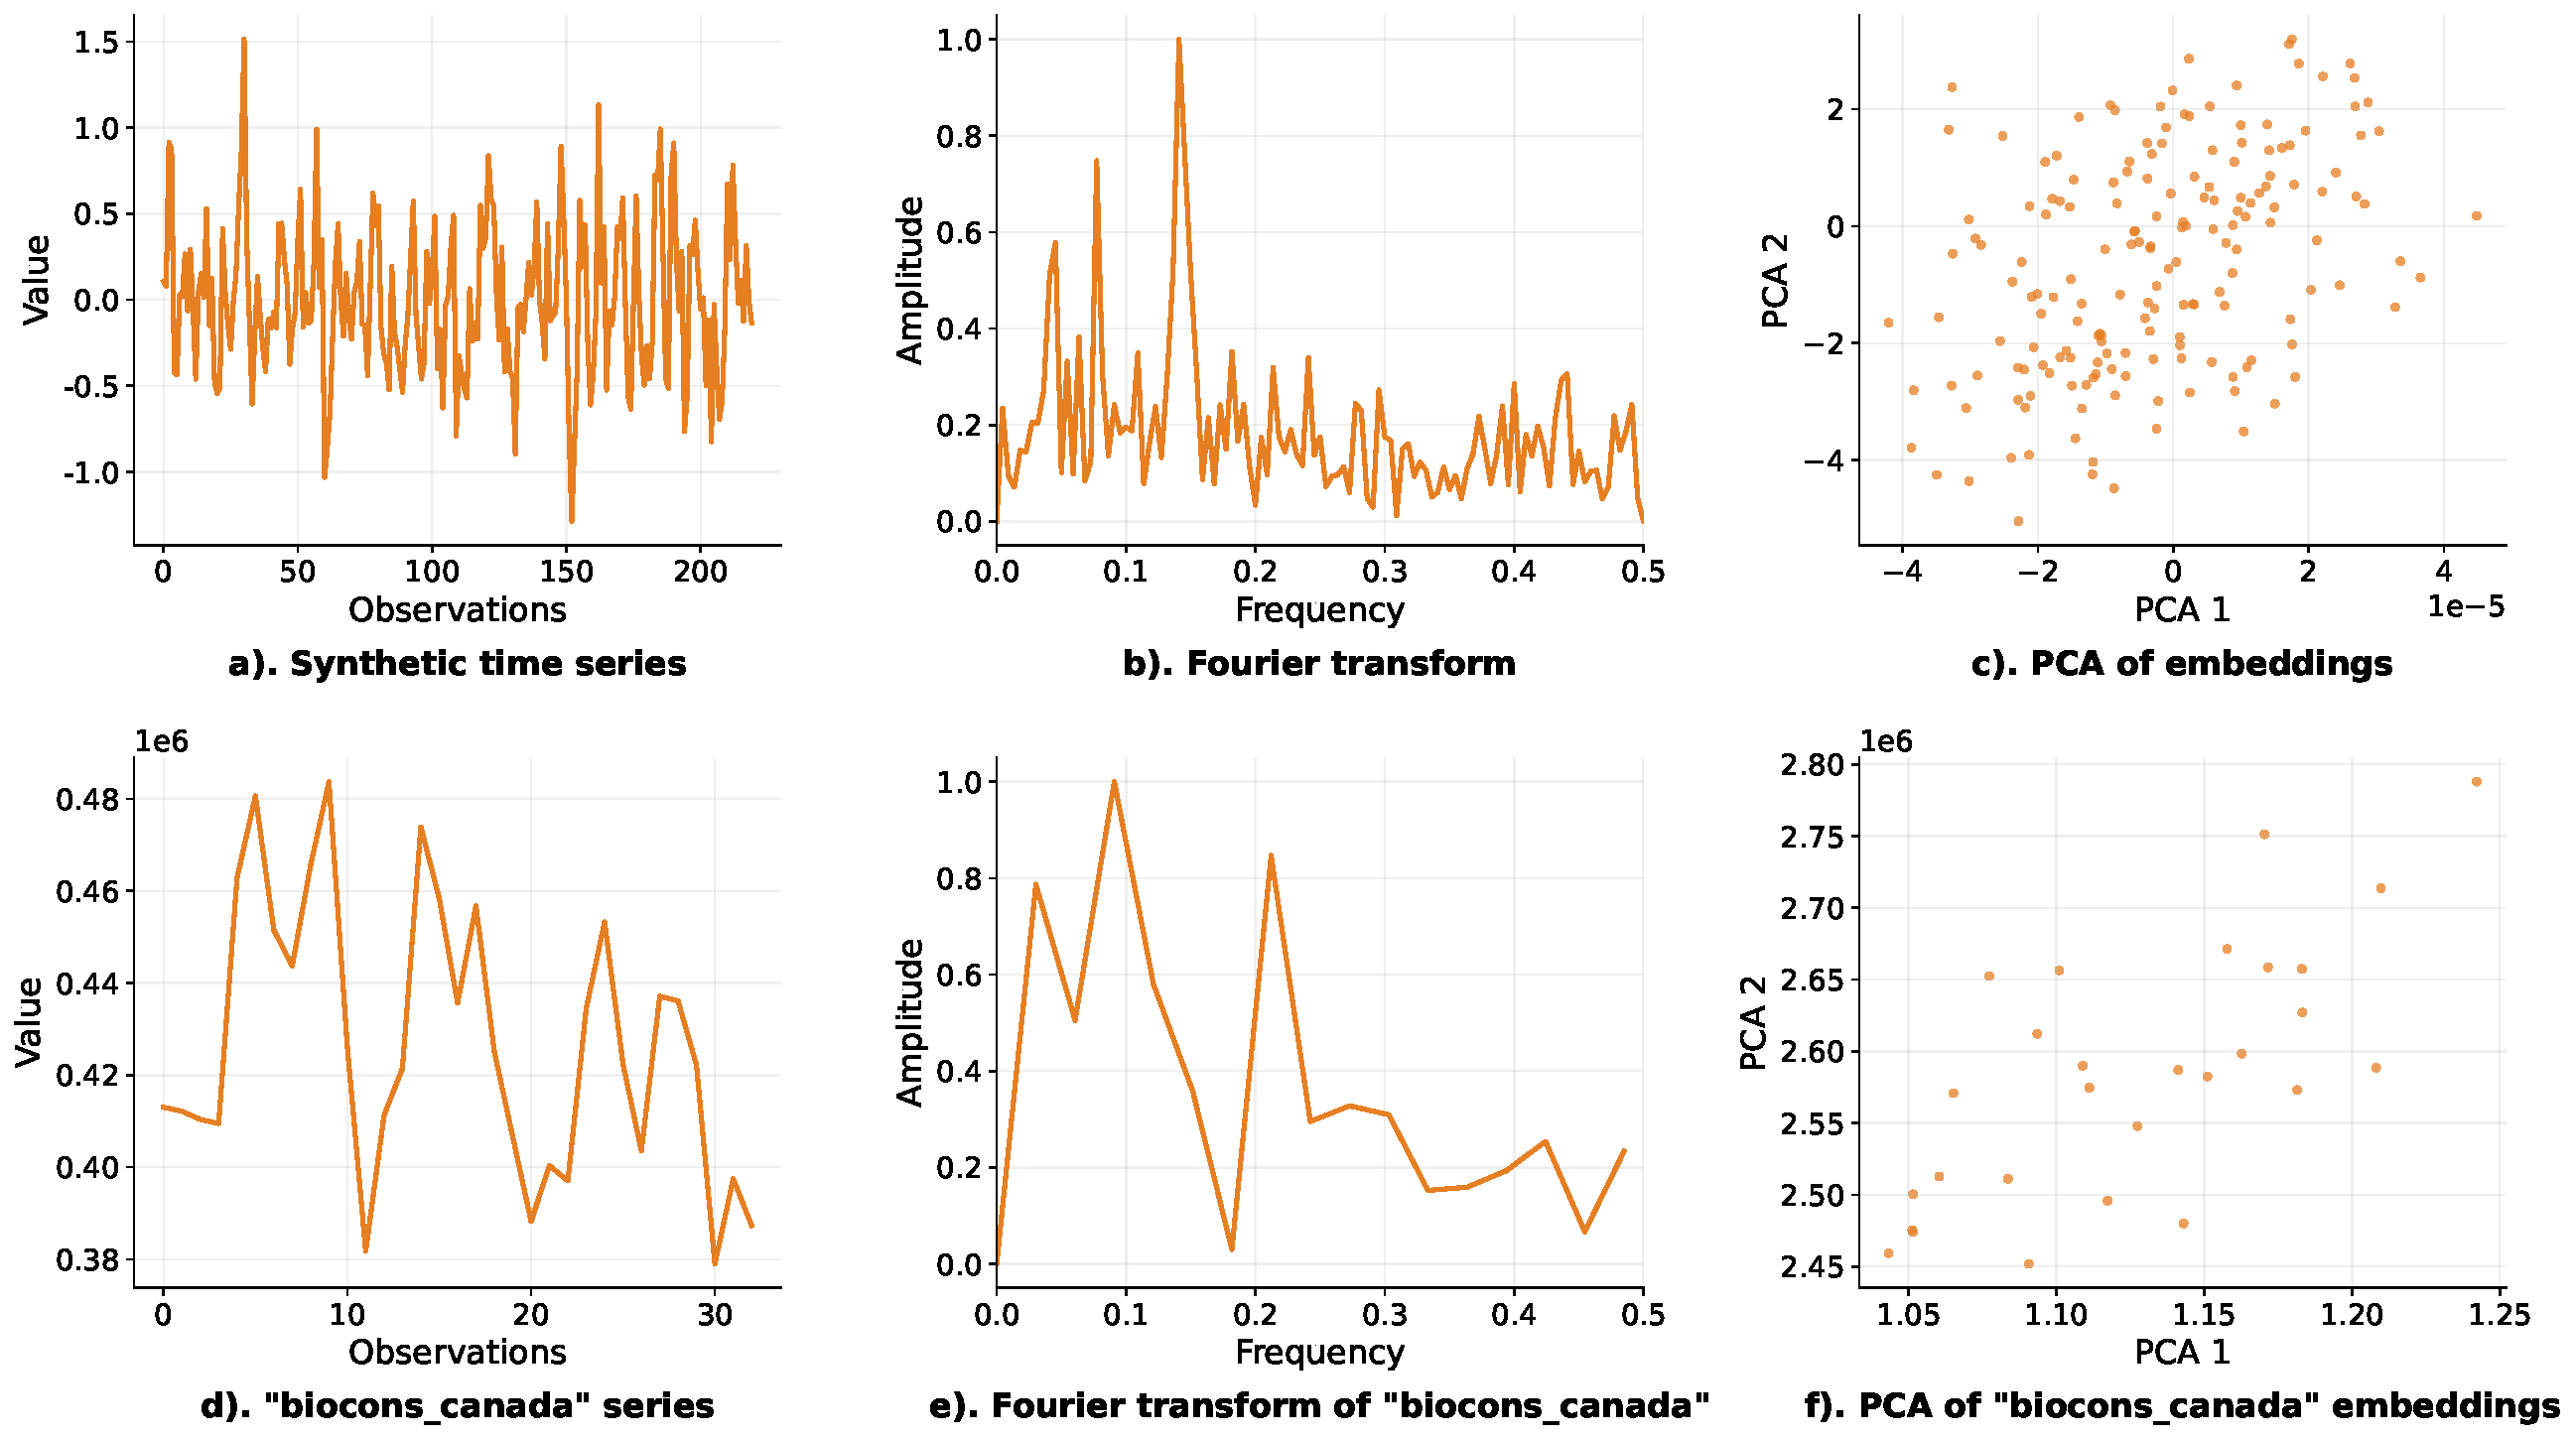
\includegraphics[width=0.95\textwidth]{fig_cluster_1.pdf}
    \caption{Characterization of series with more complex temporal behavior}
    \label{fig_cluster_1}
\end{figure*}

Complementing the individual examples, Table~\ref{tab_wilcoxon_clusters} presents Wilcoxon tests comparing ForeSight with MSRFF against ARIMA and MLP, separated by cluster and prediction type. For each comparison, we report the $p$-value, effect size, and corresponding magnitude, allowing assessment of statistical significance and practical difference between methods. The goal is to evaluate whether the performance differences observed in individual cases hold when all series in the corresponding group are considered.

In this sense, the investigation differs from the dataset-level analysis in two respects. First, series belonging to the same dataset may share temporal properties specific to that domain, favoring certain methods and enabling performance levels that do not necessarily generalize to other contexts. Second, while the dataset-level analysis considered sets of ten series, the groups defined during feature-based clustering contain substantially more series, allowing us to evaluate method behavior more broadly and independently of the domain of origin.

\begin{table*}[!ht]
\centering
\caption{Wilcoxon tests in cluster-wise comparisons}
\label{tab_wilcoxon_clusters}
\small
\renewcommand{\arraystretch}{1.25}
\setlength{\tabcolsep}{12pt}
\begin{tabular}{llccccc}
\hline
\multicolumn{1}{c}{\multirow{2}{*}[-1.0ex]{\textbf{Cluster}}} & \multicolumn{1}{c}{\multirow{2}{*}[-1.0ex]{\shortstack{\textbf{Wilcoxon} \\ \textbf{Test}}}} & \multicolumn{2}{c}{\textbf{Rolling Origin}} & & \multicolumn{2}{c}{\textbf{Steps Ahead}} \\
\cline{3-4}\cline{6-7}
& & \raisebox{-2.5ex}{\shortstack{\textbf{ForeSight} \\ \textbf{vs. ARIMA}}} & \raisebox{-2.5ex}{\shortstack{\textbf{ForeSight} \\ \textbf{vs. MLP}}} & & \raisebox{-2.5ex}{\shortstack{\textbf{ForeSight} \\ \textbf{vs. ARIMA}}} & \raisebox{-2.5ex}{\shortstack{\textbf{ForeSight} \\ \textbf{vs. MLP}}} \\[10pt]

\hline
\multirow{3}{*}{\textbf{Cluster 1}}
& $p$-value  & $10^{-5}$ & $10^{-3}$ & & $10^{-6}$ & $10^{-4}$ \\
& Effect     & 0.42 & 0.28 & & 0.43 & 0.35 \\
& Magnitude  & Moderate & Low & & Moderate & Moderate \\
\hline
\multirow{3}{*}{\textbf{Cluster 2}}
& $p$-value  & $10^{-2}$ & 0.04 & & $10^{-2}$ & 0.87 \\
& Effect     & 0.33 & 0.22 & & 0.32 & --- \\
& Magnitude  & Moderate & Low & & Moderate & --- \\
\hline
\end{tabular}
\end{table*}

In cluster 1, the comparisons of ForeSight against ARIMA and MLP are statistically significant in all configurations, with $p$-values below 0.05. Effect sizes are moderate for the comparisons with ARIMA and for MLP under SA, and low for MLP under RO. In cluster 2, the comparisons with ARIMA remain statistically significant and show moderate effect sizes. The comparison with MLP under RO is also significant, with a low effect size, whereas the SA results indicate no statistically significant difference between ForeSight and MLP.

In light of this analysis, the qualitative findings suggest that the high temporal dependence and lower spectral complexity characteristic of the more regular series favor pattern identification and reuse by the latent representation, which is consistent with the statistically significant differences observed relative to the reference methods. In more complex series, on the other hand, greater oscillation and the distribution of components across different frequencies are associated with less recurrent representations and smaller benefits from temporal encoding. In this context, ForeSight remains competitive among the three methods, even though its performance reaches levels similar to MLP in SA predictions.
The observed behavior is consistent with recent literature on latent encodings for modeling and generalization \citep{trirat_universal_2026, irani_positional_2026} and on enriched input representations for WiSARD-based networks \citep{baby_cawnn_2026}.


\section{Conclusion}
\label{sec_conclusion}


This work presents ForeSight, a new method that combines temporal encoding techniques with WNN architectures for time series forecasting. In the evaluated scenarios, ForeSight improves predictive performance relative to the baseline WNNs by operating on explicit temporal representations.

Regarding \textit{RQ1}, the results show that ForeSight is competitive with reference methods, including ARIMA, MLP, Chronos, and DL architectures, while maintaining substantially lower runtimes than more computationally demanding alternatives in the evaluated scenarios. The multiobjective analysis of accuracy and estimated energy consumption also placed it on the Pareto frontier, reinforcing its potential in scenarios where resource efficiency is relevant. Considering the datasets and ranking procedures used in forecasting competitions, ForeSight achieved the best average placement among the analyzed methods within the evaluated scenarios.

Regarding \textit{RQ2}, the results show that the temporal encoding technique affects predictive performance, with MSRFF achieving the best average ranking, while increasing the latent dimension raises computational cost. Fixed encodings remained more computationally efficient than the learned alternatives, and MSRFF provided the most favorable accuracy--efficiency trade-off among the evaluated ForeSight variants.

Regarding \textit{RQ3}, the feature-based analysis associated ForeSight's largest gains with more regular series characterized by lower spectral complexity and greater temporal dependence. The cluster-wise comparisons showed larger effect sizes for this group. For more complex series, the differences remained significant relative to ARIMA, whereas ForeSight and MLP reached comparable performance under the steps-ahead strategy.

The integration into TSPredIT complements these findings by providing a common open-source workflow for preprocessing, hyperparameter optimization, forecasting strategy definition, evaluation, and result logging. This implementation supports reproducible execution and systematic comparison of ForeSight with heterogeneous forecasting methods under the same evaluation protocol.

Among the main limitations are the growth of RAM memories due to binarization and embedding dimensionality, which may increase memory and processing consumption, and the absence of an explicit mechanism for adapting WNN memories to changes in series dynamics. These limitations are connected to the trade-off observed between representation capacity, predictive quality, and computational cost. Future investigations can explore more efficient designs, such as the incorporation of Bloom filters \citep{susskind_weightless_2022} or the adoption of differentiable WNNs \citep{bacellar_differentiable_2024}, as well as systematically evaluate ForeSight with components such as trend and seasonality modeled separately \citep{hyndman_forecasting_2021}. It is also necessary to investigate in a more controlled way the influence of characteristics such as autocorrelation, spectral complexity, noise, and structural changes on embedding selection \citep{fulcher_highly_2014}.

Another direction involves adapting ForeSight to changes in series dynamics through forgetting mechanisms \citep{cardoso_clustering_2016}, temporal decay, and change detection \citep{ogasawara_event_2025}. Finally, ensemble strategies \citep{lusquino_extending_2020} can be investigated to improve predictive performance in heterogeneous series and more complex scenarios. Overall, the results support ForeSight as an efficient and reproducible alternative for time series forecasting when predictive competitiveness and controlled computational cost are relevant requirements.

\section*{Data and code availability statement}
The source code and configurations used to reproduce the experiments are available in an online repository. The repository URL is withheld for double-anonymized review and will be provided in the final version.

\section*{Declaration of competing interest}
The authors declare that they have no known competing financial interests or personal relationships that could have appeared to influence this paper.

\section*{Declaration of generative AI and AI-assisted technologies in the writing process}
During the preparation of this work, the authors used DeepL to improve the English in the manuscript and ChatGPT to assist with code used to create graphical illustrations. After using these tools, the authors reviewed and edited the content as needed and take full responsibility for the content of the publication.


\bibliographystyle{elsarticle-harv}
\bibliography{references}

\end{document}
